\documentclass{mwart}

            % Papier
\usepackage{polski}
\usepackage[utf8]{inputenc}
\usepackage[a4paper, total={16cm, 24cm}]{geometry}

            % Matematyka
\usepackage{amsthm}
\usepackage{amsmath}
\usepackage{amssymb}

           % Wygląd
%\usepackage{url}
\usepackage{hyperref}
\usepackage{graphics}
\usepackage{fancyhdr}
\usepackage{geometry}
\usepackage{enumitem}

            % Obrazki
\usepackage{graphicx}



            % Ustawienia ramek
\usepackage[nobreak=false]{mdframed}
\mdfsetup{%
% frametitlerule=true,
% subtitlebelowline=true,
subtitleaboveline=true,
subtitleaboveskip=0,
subtitlebelowskip=0,
linewidth=1pt}


% Skroty
\newcommand{\R}{\mathbb{R}}
\newcommand{\N}{\mathbb{N}}
\newcommand{\Z}{\mathbb{Z}}
\newcommand{\C}{\mathbb{C}}
%           Pisane
\newcommand{\F}{\mathcal{F}}
\newcommand{\T}{\mathcal{T}}

\newtheorem{zad}{Zadanie}[section]

%Zmiana formatu sekcji
\renewcommand{\thesection}{\arabic{section}}


% Początek strony tytułowej


\author{\textbf{Grupa 3} \\ \textsf{Informatyka i Systemy Informacyjne | MiNI PW}}
\title{%
%\includegraphics[width=1\textwidth]{logo_uczelni.png}
\textbf{Matematyka Dyskretna I}}


%\setcounter{secnumdepth}{1}
\pagestyle{fancy}
\setlength{\headsep}{1.2cm}
\fancyhead{}
\lhead{Grupa 3\\\textsf{Wydział MiNI PW}}
\chead{\Large \textbf{Rozwiązania zadań}}
\rhead{\textbf{Matematyka Dyskretna 1}\\Informatyka}

\fancyfoot{}
\rfoot{\texttt{\thepage}}

\fancypagestyle{specialfooter}{%
    \fancyhf{}
    \renewcommand\headrulewidth{0pt}
    \fancyfoot[C]{\Large{Lato 2025}}
}


\begin{document}
\maketitle{}
\begin{center}
    Studenckie rozwiązania zadań z ćwiczeń z Matematyki Dyskretnej I. \\
    Ćwiczenia z \emph{MD I} w gr. 3 prowadzi dr inż. Tomasz Brengos \\
    i też oto pod jego opieką powstaje ten plik. \\
    Ostatnia aktualizacja: \today{} \\
    \tableofcontents
    \thispagestyle{specialfooter}

\end{center}

% Koniec strony tytułowej

















% Poczatek dokumentu
\newpage
\section{Zestaw}              % Zestaw 1
\begin{zad}[Krzysztof Wójtowicz, Autor 2]
    Na płaszczyźnie poprowadzono $n$ prostych, z których żadne dwie nie
    są równoległe i żadne trzy nie przechodzą przez ten sam punkt.
    Wyznacz liczbę:
    \begin{enumerate}
        \item obszarów, na które te proste dzielą płaszczyznę;
        \item obszarów ograniczonych, na które te proste dzielą płaszczyznę.
    \end{enumerate}
\end{zad}
\begin{mdframed}
    \begin{enumerate}
        % Rozwiązanie: Krzysztof Wójtowicz
        \item Zauważymy, że każda kolejna prosta przecina wszystkie poprzednie proste,
              a co za tym idzie również obszary, które są do nich "przyległe", dzieląc je na
              dwa. Każda poprzednia prosta ma dwa takie obszary, więc ich ogólna liczba to
              (odejmujemy obszary wspólne, czyli te "pośrodku" dwóch prostych, by ich nie duplikować):
              \[2(n-1) - (n-1-1) = n\] Zatem każda kolejna prosta dodaje n nowych obszarów:
              \[P(n) = P(n-1) + n = P(0) + \sum_{k=1}^{n} k = 1 + \frac{n(n+1)}{2}\]
              gdzie $P(n)$ to liczba obszarów dla n prostych.
              \newline
        \item Liczbę obszarów ograniczonych otrzymamy odejmując liczbę obszarów nieograniczonych z wyniku z podpunku 1.
              Każda prosta ma dwa "przyległe" obszary nieograniczone, więc liczba wszystkich takich obszarów to $2n$,
              zatem liczba wszystkich obszarów ograniczonych to:
              \[1 + \frac{n(n+1)}{2} - 2n = \frac{n^2 - 3n + 2}{2} = \frac{(n-1)(n-2)}{2}\]
    \end{enumerate}
\end{mdframed}
\begin{mdframed}
    \begin{enumerate}
        \item Rozwiązanie Autora 2 podpunktu 1
        \item Rozwiązanie Autora 2 podpunktu 2
    \end{enumerate}
\end{mdframed}



\begin{zad}[Autor 1, Autor 2]
    Ciąg Fibonacciego $\{F_n\}_{n \in \mathbb{N}}$ zadany jest przez
    $F_0=0$, $F_1=1$ i $F_{n+2}=F_{n+1}+F_n$. Udowodnij, że: \\
    \begin{enumerate}
        \item $F_0 + ... + F_n = F_{n+2} - 1$;
        \item $5|F_{5n}$,
        \item $F_n < 2_n$.
    \end{enumerate}
\end{zad}
\begin{mdframed}
    \begin{enumerate}
        \item Rozwiązanie Autora 1 podpunktu 1
        \item Rozwiązanie Autora 1 podpunktu 2
        \item Rozwiązanie Autora 1 podpunktu 3
    \end{enumerate}
\end{mdframed}
\begin{mdframed}
    \begin{enumerate}
        \item Rozwiązanie Autora 2 podpunktu 1
        \item Rozwiązanie Autora 2 podpunktu 2
        \item Rozwiązanie Autora 2 podpunktu 3
    \end{enumerate}
\end{mdframed}




\begin{zad}[Autor 1, Autor 2]
    Turniej $n$-wierzchołkowy to dowolny graf skierowany $G = (V, E)$, gdzie $|V| = n$
    i w którym $(u, v) \in E$ lub $(v, u) \in E$ dla dowolnych $u, v \in V$.
    Pokaż, że w dowolnym niepustym turnieju istnieje wierzchołek z którego można “przejść”
    po krawędziach zgodnie z ich skierowaniem do dowolnego innego wierzchołka w co
    najwyżej dwóch krokach.
\end{zad}
\begin{mdframed}
    Rozwiązanie Autora 1.
\end{mdframed}
\begin{mdframed}
    Rozwiązanie Autora 2.
\end{mdframed}

\begin{zad}[Autor 1, Autor 2]
    Udowodnij, że każdy turniej ma ścieżkę Hamiltona.
\end{zad}
\begin{mdframed}
    Rozwiązanie Autora 1.
\end{mdframed}
\begin{mdframed}
    Rozwiązanie Autora 2.
\end{mdframed}




\begin{zad}[Autor 1, Autor 2]
    W każdym polu szachownicy rozmiaru $n x n $ znajduje się jedna osoba.
    Część osób zarażona jest wirusem grypy. Wirus grypy rozprzestrzenia się w dyskretnych
    odstępach czasowych w sposób następujący:
    \begin{itemize}
        \item osoby zarażone pozostają zarażone,
        \item osoba ulega zarażeniu jeżeli co najmniej dwie sąsiadujące z nią osoby są już zarażone
              (przez osobę sąsiednią rozumiemy osobę siedzącą z przodu, z tyłu, z lewej lub prawej
              strony).
              Wykaż, że jeżeli na początku zarażonych jest istotnie mniej niż n osób, to w każdej chwili
              przynajmniej jedna osoba pozostaje niezarażona.
    \end{itemize}
\end{zad}
\begin{mdframed}
    Rozwiązanie Autora 1.
\end{mdframed}
\begin{mdframed}
    Rozwiązanie Autora 2.
\end{mdframed}




\begin{zad}[Krzysztof Wójtowicz, Autor 2]
    Wykaż, że w grupie $n$ osób istnieją dwie, które mają taką samą liczbę znajomych.
\end{zad}
\begin{mdframed}
    \underline{Dowód:}
    \newline
    W grupie $n$ osób każda osoba może mieć od $0$ do $n-1$ znajomych, ale wtedy:
    \begin{enumerate}
        \item Jeśli ktoś ma $0$ znajomych to maksymalna liczba znajomych to $n-2$, bo osoba mająca $n-1$ znajomych
              musiałaby być znajomym z osobą, która ma ich $0$, co jest niemożliwe
        \item Jeśli minimalna liczba znajomych to $1$ to wtedy maksymalna liczba znajomych to $n-1$
    \end{enumerate}
    W obydwu przypadkach mamy $n-1$ wartości oraz $n$ osób. Zatem na mocy zasady Dirichleta conajmniej dwie
    osoby muszą mieć tę samą liczbę znajomych.
    $\blacksquare$
\end{mdframed}
\begin{mdframed}
    Rozwiązanie Autora 2.
\end{mdframed}




\begin{zad}[Autor 1, Autor 2]
    Przy okrągłym stole jest $n$ miejsc oznaczonych proporczykami różnych
    państw. Ambasadorowie tych państw usiedli przy tym stole tak, że żaden z nich nie siadł
    przy właściwym proporczyku. Wykaż, że można tak obrócić stołem, że co najmniej 2
    ambasadorów znajdzie się przed proporczykiem swojego państwa.
\end{zad}
\begin{mdframed}
    Rozwiązanie Autora 1.
\end{mdframed}
\begin{mdframed}
    Rozwiązanie Autora 2.
\end{mdframed}




\begin{zad}[Autor 1, Autor 2]
    Pokaż, że w dowolnym ciągu n liczb całkowitych istnieje (niepusty)
    podciąg kolejnych elementów taki, że suma wyrazów podciągu jest wielokrotnością n.
\end{zad}
\begin{mdframed}
    Rozwiązanie Autora 1.
\end{mdframed}
\begin{mdframed}
    Rozwiązanie Autora 2.
\end{mdframed}




\begin{zad}[Autor 1, Autor 2]
    Rozważ dowolną rodzinę podzbiorów zbioru $n$--elementowego zawierającą
    więcej niż połowę wszystkich podzbiorów. Wykaż, że w tej rodzinie muszą być dwa zbiory
    takie, że jeden zawiera się w drugim.
\end{zad}
\begin{mdframed}
    Rozwiązanie Autora 1.
\end{mdframed}
\begin{mdframed}
    Rozwiązanie Autora 2.
\end{mdframed}



\begin{zad}[Autor 1, Autor 2]
    Dla $n$--elementowego zbioru $X$ rozważ pewną rodzinę jego podzbiorów
    $\mathcal{F}$, gdzie $|F| > n/2$ dla każdego $F \in \mathcal{F}$. Wykaż, że istnieje
    $x \in X$ należący do co najmniej połowy zbiorów z $\mathcal{F}$.
\end{zad}
\begin{mdframed}
    Rozwiązanie Autora 1.
\end{mdframed}
\begin{mdframed}
    Rozwiązanie Autora 2.
\end{mdframed}


\begin{zad}[Autor 1, Autor 2]
    Dana jest kwadratowa szachownica $n \times n$. Dla jakich wartosci $n\geq 1$
    możemy pokryć tę szachownicę kostkami wielkości $2 \times 2$ oraz $3 \times 3$.
\end{zad}
\begin{mdframed}
    Rozwiązanie Autora 1.
\end{mdframed}
\begin{mdframed}
    Rozwiązanie Autora 2.
\end{mdframed}


\begin{zad}[Autor 1, Autor 2]
    Dana jest kwadratowa szachownica $2n \times 2n$ z wyciętym jednym polem.
    Wykaż, że dla wszystkich wartości $n \geq 1$ możemy pokryć tę szachownicę kostkami w
    kształcie litery L (czyli kwadrat $2 \times 2$ bez jednego pola).
\end{zad}
\begin{mdframed}
    Rozwiązanie Autora 1.
\end{mdframed}
\begin{mdframed}
    Rozwiązanie Autora 2.
\end{mdframed}






















\newpage
\section{Zestaw}          % ZESTAW 2

\begin{zad}[Filip Sajko, Bartłomiej Sokołowski]
    Na ile sposobów można ustawić $n$ wież na szachownicy
    $n \times n$ tak, by żadne dwie nie znajdowały się w
    polu wzajemnego rażenia.
\end{zad}
\begin{mdframed}
    Starczy zauważyć, że dla każdej wieży wybieramy rząd i kolumnę
    w której się znajduje -- i tym samym zmniejsza liczbę dostępnych
    o jeden. Tak więc odpowiedź wynosi: \[n \cdot n \cdot (n-1) \cdot
        (n-1) \cdot ... \cdot 2 \cdot 2 \cdot 1 \cdot 1 =  n! \cdot n!\]
\end{mdframed}
\begin{mdframed}
    %Rozwiązanie: Bartłomiej Sokołowski
    Musimy wybrać $n$ pozycji z $n^2$ dostępnych pól na szachownicy. Wybierając
    $1$ pozycję automatycznie eliminujemy całą kolumnę oraz wiersz, w którym znajduje się wybrane pole.
    \item Pierwszą wieżę wybieramy z $n \times n = n^2$ dostępnych pozycji.
    \item Następną wieżę wybieramy na $(n-1) \times (n-1) = (n-1)^2$ sposobów, ponieważ wykluczamy wybraną już kolumnę i wiersz.
    \item Powtarzając proces $n$ razy dostajemy:
    \[n \times n \times (n-1) \times (n - 1) \times ... \times 1 \times 1 = n! \times n! = (n!)^2\]
\end{mdframed}




\begin{zad}[Filip Sajko, Autor 2]
    Na ile sposobów można ustawić $k$ wież na szachownicy $n \times m$
    tak, by żadne dwie nie znajdowały się w polu wzajemnego rażenia.
\end{zad}
\begin{mdframed}
    Zadanie analogiczne od poprzedniego - z tym, że zmienił nam się
    rozmiar planszy, a ponadto nie wypełniamy jej całej. Zasada
    pozostaje jednak ta sama. Na start jednak warto założyć, że
    $k \leq max\{n, m\}$ (choć w sumie jeżeli tak nie jest, to
    odpowiedź to 0). Mając to już za sobą:
    \[n \cdot m \cdot (n-1) \cdot (m-1) \cdot ... \cdot (n - k +1) \cdot (m -k +1)\]
    (wykonujemy mnożenie $k + k$ elementów -- stąd to $-k + 1$).
\end{mdframed}
\begin{mdframed}
    Rozwiązanie Autora 2.
\end{mdframed}




\begin{zad}[Filip Sajko, Autor 2]
    Znaleźć definicje rekurencyjne następujących ciągów:
    \begin{enumerate}
        \item $a(n)$ -- liczba słów długości $n$ nad alfabetem
              $\{0, 1\}$, które nie zawierają dwóch jedynek koło siebie.
        \item  $b(n)$ -- liczba różnych pokryć prostokąta o wymiarze
              $2 \times n$ dominami wymiaru $2 \times 1$.
    \end{enumerate}
\end{zad}
\begin{mdframed}
    \begin{enumerate}

        \item Oczywiście $a(1)=2$, $a(2)=3$.  Rozważmy słowo $n$ elementowe.
              Zauważamy, że jeżeli ono kończy sie ono zerem to poprzedzające słowo $n-1$
              elementowe jest dowolne. Jeżeli natomiast kończy się jedynką,
              to poprzedzające słowo $n-2$ elementowe jest dowolne
              (tak jakby cofamy się krok dalej by mieć dowolność).
              Stąd: $a(n)=a(n-1)+a(n-2)$.
        \item Analogicznie do poprzedniego. Jak wiemy $a(1) = 1$, $a(2) = 2$. Zastanówmy się nad $a(n)$:
              Rozważamy ciąg o długości $n$. Jeżeli na końcu jest blok poziomy,
              to wiemy że powstał on z ciągu długości $a(n-2)$.
              Jeżeli jest pionowy, to wiemy, że musiał on powstać z ciągu długości $n-1$.
              A stąd $a(n) = a(n-1) + a(n-2)$.
    \end{enumerate}
\end{mdframed}
\begin{mdframed}
    Rozwiązanie Autora 2.
\end{mdframed}




\begin{zad}[Autor 1, Autor 2]
    Ile rozwiązań ma równanie $x_1 + x_2+x_3+x_4 = 7$:
    \begin{enumerate}
        \item gdzie $x_i$ są liczbami naturalnymi?
        \item gdzie $x_i$ są dodatnimi liczbami naturalnymi?
    \end{enumerate}
\end{zad}
\begin{mdframed}
    \begin{enumerate}
        \item Rozwiązanie Autora 1 podpunktu 1
        \item Rozwiązanie Autora 1 podpunktu 2
    \end{enumerate}
\end{mdframed}
\begin{mdframed}
    \begin{enumerate}
        \item Rozwiązanie Autora 2 podpunktu 1
        \item Rozwiązanie Autora 2 podpunktu 2
    \end{enumerate}
\end{mdframed}




\begin{zad}[Autor 1, Autor 2]
    Rozważmy czekoladę złożoną z $m\times n$ kostek.
    Na ile sposobów można wykroić prostokąt złożony z $k \times k$
    sąsiadujących ze sobą kostek czekolady?
\end{zad}
\begin{mdframed}
    Rozwiązanie Autora 1.
\end{mdframed}
\begin{mdframed}
    Rozwiązanie Autora 2.
\end{mdframed}




\begin{zad}[Maciej Wełpa, Autor 2]
    (Reguła sumowania po górnym indeksie). Udowodnij, że dla
    $n, k \in \mathbb{N}$ zachodzi
    \[\sum_{j=0}^n\binom{j}{k} = \binom{n+1}{k+1}\]
\end{zad}
\begin{mdframed}
    % Rozwiązanie: Maciej Wełpa
    \textbf{Lewa strona:}
    Niech X to zbiór wszystkich k + 1 elementów z ze zbioru n + 1 elementów, \\
    \(|X|\) = \(\binom{n + 1}{k + 1}\). \\
    \textbf{Prawa strona:} Niech \( X_j \) to podzbiory \(|k+1|\) elementowe ze zbioru X, które
    zawierają maksymalny element j+1. np. dla k = 2 \( X_3 \) = \{1, 2, 4\}, \( X_4 \) = \{1, 3, 5\}
    - ostatni element jest największy, pozostałe dwa to wybrane z \{1...j\}. Rozważamy j elementów mniejszych od j+1, spośród nich wybieramy k elementów - mamy \(\binom{j}{k}\) możliwości. Sumując po j dodajemy do siebie wszystkie możliwości.
\end{mdframed}
\begin{mdframed}
    Rozwiązanie Autora 2.
\end{mdframed}




\begin{zad}[Bartłomiej Sokołowski, Autor 2]
    (Reguła sumowania równoległego). Udowodnij, że dla $n, k \in \mathbb{N}$
    zachodzi \[ \sum_{j= 0}^{n}\binom{n+j}{j} = \binom{n+k+1}{k}   \]
\end{zad}\
\begin{mdframed}
    %Rozwiązanie: Bartłomiej Sokołowski 
    Przeprowadzimy dowód indukcyjny.
    \item k = 0:
    \item \[ L = \sum_{j=0}^{0}\binom{n+j}{j} = \binom{n}{0} = 0 \]
    \item \[P = \binom{n+0+1}{0} = \binom{n+1}{0} = 0\]
    \item Zał. indukcyjne :
    \item \[\sum_{j=0}^{k}\binom{n+j}{j} = \binom{n+k+1}{k}\]
    \item Teza indukcyjna :
    \item \[\sum_{j=0}^{k+1}\binom{n+j}{j} = \binom{n+k+2}{k+1}\]
    \item \[\sum_{j=0}^{k+1}\binom{n+j}{j} = \sum_{j=0}^{k}\binom{n+j}{j} + \binom{n+k+1}{k+1} = \binom{n+k+1}{k} + \binom{n+k+1}{k+1} = \binom{n+k+2}{k+1}\]
\end{mdframed}
\begin{mdframed}
    Rozwiązanie Autora 2.
\end{mdframed}



\begin{zad}[Krzysztof Wojczakowski, Autor 2]
    Ile jest funkcji $f:\{1, ..., n\} \to \{1, ..., n\}$ monotonicznych takich,
    że $f(i) \leq f(j) $ dla $i < j$?
\end{zad}
\begin{mdframed}
    %Rozwiązanie: Krzysztof Wojczakowski
    Zauważmy, że te funkcje tworza tak jakby jakby ciąg , który ma być niemalejący.
    Możemy to zobrazować jako kratę gdzie wartości na dole to liczby od 1 do n , a idąc do góry
    mozemy tylko iść w prawo lub w górę. , gdie tyle ile kresek w górę przy danej liczbie to tyle ile razy tą liczbę wybieramy.
    \vspace{0.3em} % mały odstęp w pionie

    \noindent
    \centering
    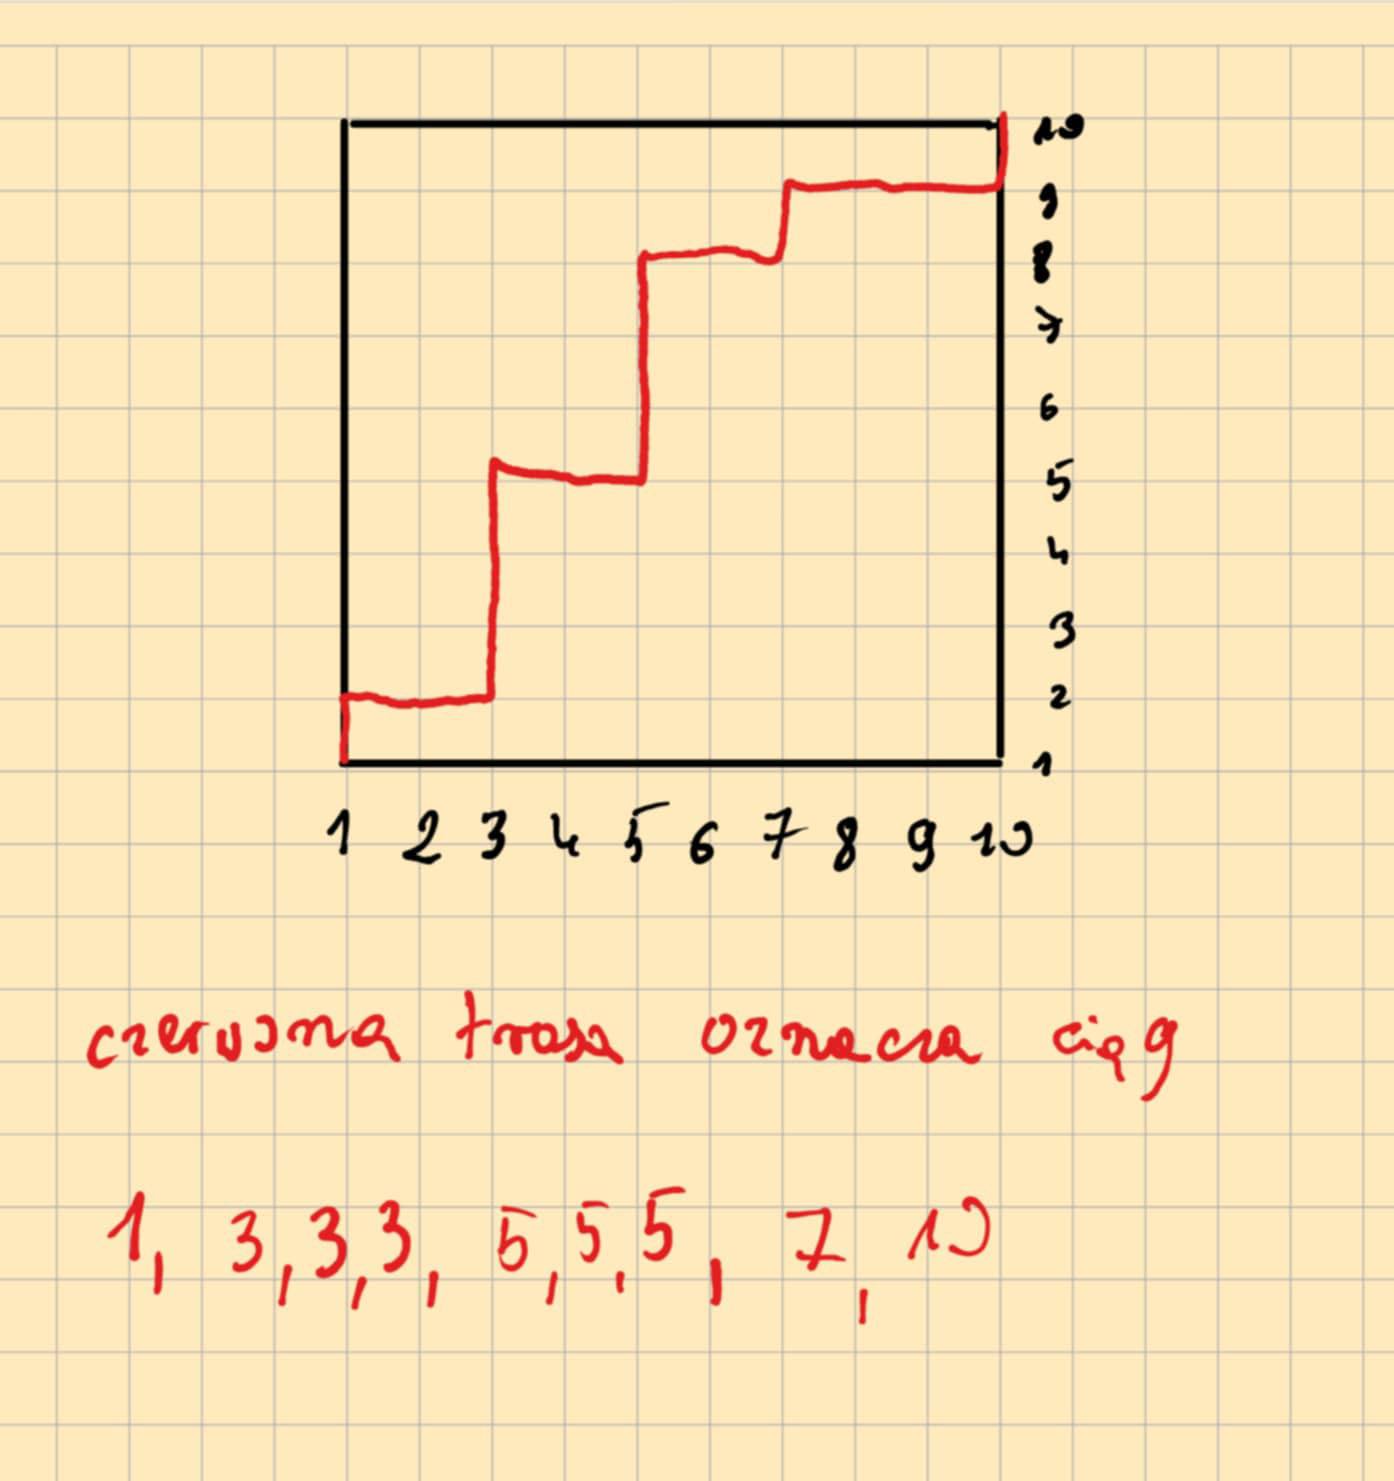
\includegraphics[width=0.7\textwidth]{images/zadanie28.png}

    Końcowo poszliśmy $n-1$ razy w prawo i $n-1$ razy w górę, czyli mamy $n-1+n-1 = 2n - 2$ kroków
    W rezultacie takich funkcji jest:
    \( \binom{2n-2}{n-1} \)
\end{mdframed}
\begin{mdframed}
    Rozwiązanie Autora 2.
\end{mdframed}




\begin{zad}[Krzysztof Wojczakowski, Autor 2]
    Ile jest $k$--elementowych podzbiorów zbioru $n$--elementowego, które nie
    zawierają dwóch sąsiednich liczb?
\end{zad}
\begin{mdframed}
    %Rozwiązanie: Krzysztof Wojczakowski
    Zauważmy, że jeżeli mamy mamy do wybrania $k$ elementow , to równolegle to oznacza , że
    musimy zrobić $k-1$ "przerw" pomiędzy nimi. Wygląda to tak:
    \verb|_0_0_0_..._0_0_|
    gdzie zero to oznacza ze liczby nie bierzemy, a podłoga oznacza, że bierzemy.
    Zostaje nam $n-(k+1)$ miejsc do wyboru, czyli $n-k+1$ miejsc.
    w takim razie ilość $k$ elementowych podzbiorów jest :
    \( \binom{n-k+1}{k} \)

\end{mdframed}
\begin{mdframed}
    Rozwiązanie Autora 2.
\end{mdframed}


\begin{zad}[Autor 1, Autor 2]
    Posługując się interpretacją kombinatoryczną udowodnij, że:
    \[ \sum_{i=0}^{k} \binom{n}{i} \binom{n-i}{k-i} = 2^k \binom{n}{k} \]
\end{zad}
\begin{mdframed}
    Rozwiązanie Autora 1.
\end{mdframed}
\begin{mdframed}
    Rozwiązanie Autora 2.
\end{mdframed}




\begin{zad}[Katarzyna Szwed, Mateusz Rabantek]
    Udowodnij poniższe tożsamości na dwa sposoby: posługując się interpretacją
    kombinatoryczną albo rozwinięciem dwumianu $(1 + x)^n$:
    \begin{enumerate}
        \item \[\sum_{k=0}^{n}k\binom{n}{k} = n2^{n-1}\]
        \item \[\sum_{k=0}^{n}k^2\binom{n}{k}= (n+n^2)2^{n-2}\]
        \item \[\sum_{i=0}^{k}\binom{m}{i}\binom{n}{k-i} = \binom{m+n}{k} \]
    \end{enumerate}
\end{zad}
\begin{mdframed}
    %Rozwiązanie: Katarzyna Szwed
    \begin{enumerate}
        \item Podpunkt 1

              Rozważmy zbiór $X$ taki, że:
              \[X := \{ (A, x) : x \in A \wedge A \subset [n]\}\]

              Żeby policzyć jego moc najpierw wybierzemy element $x \in [n]$ na $n$ sposobów,
              a potem resztę elementów zbioru $A$, czyli dowolny podzbiór $[n]-\{x\}$
              \[|X| = n \cdot 2^{n-1}\]

              Teraz rozważmy rodzinę zbiorów $\{X_k\}_{k=0}^n$:
              \[X_k := \{(A, x) \in X : |A| = k\}\]

              Żeby policzyć moc zbioru $X_k$ (dla danego $k$) najpierw wybieramy $k$-elementowy zbiór $A$ będący podzbiorem $[n]$, a potem należący
              do niego element $x$:
              \[|X_k| = {n \choose k} \cdot k\]

              Rodzina $X_k$ jest rozłącznym pokryciem zbioru $X$, zatem mamy:
              \[|X| = \sum_{k=0}^{n} |X_k|\]
              \[n \cdot 2^{n-1} = \sum_{k=0}^{n} k \cdot {n \choose k}\]

        \item Podpunkt 2

              Rozważmy zbiór $X$ taki, że:
              \[X := \{(A, x_1, x_2) : A \subset [n] \wedge x_1, x_2 \in A\}\]

              Żeby policzyć moc zbioru $X$ osobno policzymy przypadki kiedy $x_1 = x_2$ i $x_1 \neq x_2$.

              Dla $x_1 = x_2$ wybieramy najpierw wyróżniony element na $n$ sposobów, a potem dobieramy resztę elementów z $A$,
              dostajemy $n2^{n-1}$.

              Dla $x_1 \neq x_2$ wybieramy $x_1$ na $n$ sposobów, $x_2$ na $n-1$ sposobów, a potem dobieramy resztę elementów z $A$,
              dostajemy $n(n-1)2^{n-2}$.
              Zatem mamy:
              \[|X| = n2^{n-1} + n(n-1)2^{n-2} = (2n + n^2 - n)2^{n-2} = (n + n^2)2^{n-2}\]

              Teraz rozważmy rodzinę zbiorów $\{X_k\}_{k=0}^n$:
              \[X_k := \{(A, x_1, x_2) \in X : |A| = k\}\]

              Żeby policzyć moc zbioru $X_k$ (dla danego $k$) najpierw wybierzemy $k$-elementowy zbiór $A \subset [n]$, a potem wybierzemy z niego elementy
              $x_1$ i $x_2$ (przy czym mogą być one sobie równe):
              \[|X_k| = {n \choose k} \cdot k\cdot k\]

              Rodzina $X_k$ jest rozłącznym pokryciem zbioru $X$, więc otrzymujemy:
              \[\sum_{k=0}^{n} |X_k| = |X|\]
              \[\sum_{k=0}^{n}k^2{n \choose k}= n(n+1)2^{n-2}\]

        \item Podpunkt 3

              Rozważmy zbiór $X$ taki, że:
              \[X := \{A \subset [m + n] : |A| = k\}\]

              Zauważmy, że $|X| = {m+n \choose k}$.

              Teraz rozważmy rodzinę zbiorów $\{X_i\}_{i=0}^n$:
              \[X_i := \{A \in X : |A \cap [m]| = i\}\]

              Żeby policzyć moc zbioru $X_i$ (dla danego $i$) najpierw wybieramy $i$ elementów z $[m]$, a potem $k-i$ elementów z
              $\{m+1, m+2, ..., m+n\}$, zatem $|X_i| = {m \choose i}{n \choose k-i}$.

              Rodzina $X_i$ jest rozłącznym pokryciem zbioru $X$, więc otrzymujemy:
              \[|X| = \sum_{i=0}^{n} |X_i|\]
              \[{m+n \choose k} = \sum_{i=0}^{k}{m \choose i}{n \choose k-i}\]

    \end{enumerate}
\end{mdframed}
\begin{mdframed}
    \begin{enumerate}
        %rozwiązanie: Mateusz Rabantek
        \textbf{Podpunkt 1:}

        Zacznijmy od rozwinięcia dwumianu Newtona:
        \begin{equation}
        (1+x)^n = \sum_{k=0}^{n} \binom{n}{k} x^k
        \end{equation}

        Różniczkujemy obie strony względem $x$:
        \begin{equation}
        \frac{d}{dx}(1+x)^n = \frac{d}{dx}\sum_{k=0}^{n} \binom{n}{k} x^k
        \end{equation}

        \begin{equation}
        n(1+x)^{n-1} = \sum_{k=0}^{n} k \binom{n}{k} x^{k-1}
        \end{equation}

        Podstawiamy $x = 1$:
        \begin{equation}
        n \cdot 2^{n-1} = \sum_{k=0}^{n} k \binom{n}{k} \cdot 1^{k-1} = \sum_{k=0}^{n} k \binom{n}{k}
        \end{equation}

        Zatem:
        \begin{equation}
        \boxed{\sum_{k=0}^{n} k \binom{n}{k} = n2^{n-1}}
        \end{equation}
        \newline
        \textbf{Podpunkt 2:}

        Z podpunktu 1 wiemy, że:
        \begin{equation}
        n(1+x)^{n-1} = \sum_{k=0}^{n} k \binom{n}{k} x^{k-1}
        \end{equation}

        Mnożymy obie strony przez $x$:
        \begin{equation}
        nx(1+x)^{n-1} = \sum_{k=0}^{n} k \binom{n}{k} x^k
        \end{equation}

        Różniczkujemy obie strony względem $x$:
        \begin{equation}
        \frac{d}{dx}[nx(1+x)^{n-1}] = \frac{d}{dx}\sum_{k=0}^{n} k \binom{n}{k} x^k
        \end{equation}

        \begin{equation}
        n(1+x)^{n-1} + nx(n-1)(1+x)^{n-2} = \sum_{k=0}^{n} k^2 \binom{n}{k} x^{k-1}
        \end{equation}

        Podstawiamy $x = 1$:
        \begin{equation}
        n \cdot 2^{n-1} + n(n-1) \cdot 2^{n-2} = \sum_{k=0}^{n} k^2 \binom{n}{k}
        \end{equation}

        Upraszczamy lewą stronę:
        \begin{align}
        n \cdot 2^{n-1} + n(n-1) \cdot 2^{n-2} &= n \cdot 2^{n-2} \cdot 2 + n(n-1) \cdot 2^{n-2} \\
        &= 2^{n-2}[2n + n(n-1)] \\
        &= 2^{n-2}[2n + n^2 - n] \\
        &= 2^{n-2}(n + n^2)
        \end{align}

        Zatem:
        \begin{equation}
        \boxed{\sum_{k=0}^{n} k^2 \binom{n}{k} = (n + n^2)2^{n-2}}
        \end{equation}
        \newline

        \textbf{Podpunkt 3:}

        Rozważmy iloczyn dwóch rozwinięć dwumianowych:
        \begin{equation}
        (1+x)^m \cdot (1+x)^n = (1+x)^{m+n}
        \end{equation}

        Lewa strona:
        \begin{equation}
        (1+x)^m \cdot (1+x)^n = \left(\sum_{i=0}^{m} \binom{m}{i} x^i\right) \cdot \left(\sum_{j=0}^{n} \binom{n}{j} x^j\right)
        \end{equation}

        Przy mnożeniu tych sum, współczynnik przy $x^k$ otrzymujemy jako sumę wszystkich iloczynów postaci $\binom{m}{i} \binom{n}{j}$, gdzie $i + j = k$. Oznacza to, że $j = k - i$, więc:

        Współczynnik przy $x^k$ w lewej stronie:
        \begin{equation}
        \sum_{i=0}^{k} \binom{m}{i} \binom{n}{k-i}
        \end{equation}

        Prawa strona:
        \begin{equation}
        (1+x)^{m+n} = \sum_{k=0}^{m+n} \binom{m+n}{k} x^k
        \end{equation}

        Współczynnik przy $x^k$ w prawej stronie to $\binom{m+n}{k}$.

        Porównując współczynniki przy $x^k$ w obu stronach równania:
        \begin{equation}
        \boxed{\sum_{i=0}^{k} \binom{m}{i} \binom{n}{k-i} = \binom{m+n}{k}}
        \end{equation}
    \end{enumerate}
\end{mdframed}






















\newpage
\section{Zestaw}          % ZESTAW 3

\begin{zad}[Autor 1, Autor 2]
    Wykaż, że dla dowolnego $n \geq 1$ istnieje $k \geq 1$ takie, że:
    \[S(n, 0) < S(n, 1) < ... < S(n, k - 1 ) \leq S(n, k) > S(n, k+1) > ... > S(n, n)\]
\end{zad}
\begin{mdframed}
    Rozwiązanie Autora 1.
\end{mdframed}
\begin{mdframed}
    Rozwiązanie Autora 2.
\end{mdframed}





\begin{zad}[Bartłomiej Sokołowski , Autor 2]
    Wykaż, że:
    \[B(n) = \sum_{i=0}^{n-1} \binom{n-1}{i}B(i)\]
\end{zad}
\begin{mdframed}
    %Rozwiązanie: Bartłomiej Sokołowski 
    \item Dowód:
    \item Niech $X = \pi([n])$, wtedy $|X| = B(n)$
    \item Niech $X_i = \{\pi([n]) : \exists_{A \in \pi([n])} (n \in A \land |A| = i + 1)\}$
    \item Jest to zbiór wszystkich podziałów, które zawierają n oraz mają wielkość i+1
    \item Jest to rozłączne pokrycie zbioru X
    \item \[ |X_i| = \binom{n-1}{i} \times B(n-i-1)\]
    \item gdzie $\binom{n-1}{i}$ reprezentuje wybór $i$ elementów z bloku z $n$, a $B(n-i-1)$ reprezentuje podzielenie pozostałych elementów na bloki.
    \item \[ |X| = \sum_{i=0}^{n-1} |X_i| = \sum_{i=0}^{n-1}\binom{n-1}{i} \times B(n-i-1) = \sum_{i=0}^{n-1} \binom{n-1}{n-i-1} \times B(n-i-1) = \sum_{i=0}^{n-1} \binom{n-1}{i} \times B(i)\]
    \item Ostatnie przejście to sumowanie ale od drugiej strony, dlatego można je wykonać.
\end{mdframed}
\begin{mdframed}
    %Rozwiązanie: Karol Wójcik
    Z lewej strony mamy liczbę podziałów zbioru n-elementowego na niepuste podzbiory, czyli $B(n)$
    \newline \newline
    Spróbujmy uzyskać tą liczbę w inny sposób, najpierw utworzymy blok $k+1$ elementowy, który będzie
    zawierał element $n$, a pozostałe elementy podzielimy na dowolny niepusty podzbiór:
    \newline \newline
    Weźmy zbiór $n-1$ elementowy. Wybieramy z niego $k$ elementów, co można zrobić na $\binom{n-1}{k}$
    sposobów. Następnie dołączamy do wybranych elementów element $n$. Pozostałe $n-k-1$ elementów
    możemy podzielić na $B(n-k-1)$ sposobów
    \newline
    Sumując po $k$:
    \newline \newline
    \[B(n) = \sum_{k=0}^{n-1}B{(n-k-1)}\binom{n-1}{k} \]

    Zmieńmy sumowanie na $i=n-k-1$:
    \[\sum_{i=0}^{n-1}B(i)\binom{n-1}{n-1-i} = \sum_{i=0}^{n-1}B(i)\binom{n-1}{i} \]
    \newline
    Otrzymaliśmy w ten sposób prawą stronę tezy, więc
    \newline
    \[B(n) = \sum_{i=0}^{n-1} \binom{n-1}{i}B(i)\]
\end{mdframed}




\begin{zad}[Karol Wójcik, Autor 2]
    Wykaż, że dla $n, k \in \mathbb{N}$ zachodzi:
    \[S(n,k+1)=\frac{1}{(k+1)!} \sum_{0<i_0<...<i_{k-1}<n} \binom{n}{i_{k-1}}\binom{i_{k-1}}{i_{k_2}}...\binom{i_1}{i_0}     \]
\end{zad}
\begin{mdframed}
    % Rozwiązanie: Karol Wójcik
    Zapiszmy tezę jako:
    \[(k+1)! \cdot S(n,k+1) = \sum_{0<i_0<...<i_{k-1}<n} \binom{n}{i_{k-1}}\binom{i_{k-1}}{i_{k_2}}...\binom{i_1}{i_0} \]
    \newline \newline
    Lewa strona tezy przedstawia liczbę sposobów podziału zbioru n-elementowego na $k+1$ niepustych,
    uporządkowanych podzbiorów. $S(n,k+1)$ zlicza liczbę podziałów na $k+1$ nieuporządkowanych podzbiorów,
    a mnożenie przez $(k+1)!$ nadaje tym podzbiorom kolejność.
    \newline \newline
    Spróbujmy skonstruować to w inny sposób. Rozważmy ściśle rosnący ciąg liczb całkowitych $i_0$, $i_1$ $\dots$,$i_{k-1}$,
    taki, że $0<$ $i_0$ oraz $i_{k-1}$ $<n$
    Teraz wybierzmy $i_{k-1}$ elementów ze zbioru n-elementowego. Można to zrobić na $\binom{n}{i_{k-1}}$ sposobów,
    następnie z tego wybranego zbioru $i_{k-1}$ elementowego wybieramy $i_{k-2}$ elementów na $\binom{i_{k-1}}{i_{k-2}}$ sposobów.
    Kontynuujemy ten proces, aż ze zbioru $i_1$ elementowego wybierzemy $i_0$ elementów na $\binom{i_1}{i_0}$ sposobów.
    W ten sposób uzyskujemy łańcuch zagnieżdżonych podzbiorów:
    \newline
    \[[i_0]\subset [i_1]\subset \dots \subset [i_{k-1}] \subset [n] \]
    \newline
    gdzie $|[i_j]| = i_j$
    \newline
    Taki łańcuch podzbiorów to uporządkowana kolekcja $k+1$ rozłącznych, niepustych podzbiorów zbioru $[n]$.
    Iloczyn $\binom{n}{i_{k-1}}\binom{i_{k-1}}{i_{k_2}}...\binom{i_1}{i_0}$ zlicza liczbę sposobów przeprowadzania tej sekwencji wyborów.
    Sumując po wszystich możliwych ciągach $i_0$, $i_1$ $\dots$,$i_{k-1}$ otrzymujemy
    \newline
    \[\sum_{0<i_0<...<i_{k-1}<n} \binom{n}{i_{k-1}}\binom{i_{k-1}}{i_{k_2}}...\binom{i_1}{i_0} \]
    \newline
    co obejmuje wszystkie możliwe sposoby podziały zbioru $[n]$ na $k+1$ niepustych, uporządkowanych podzbiorów.
    \newline
    Zatem prawa strona również zlicza liczbę sposobów podziału zbioru n-elementowego na $k+1$ niepustych, uporządkowanych podzbiorów.
    \newline
    Zatem
    \newline
    \[(k+1)! \cdot S(n,k+1) = \sum_{0<i_0<...<i_{k-1}<n} \binom{n}{i_{k-1}}\binom{i_{k-1}}{i_{k_2}}...\binom{i_1}{i_0} \]
\end{mdframed}
\begin{mdframed}
    Rozwiązanie Autora 2.
\end{mdframed}





\begin{zad}[Autor 1, Autor 2]
    Rozważ  następującą procedurę generującą pewne liczby naturalne
    $\{a_{i,j}\}_{1 \geq i \geq j}$:
    \begin{enumerate}
        \item $a_{0,0} = 1$,
        \item $a_{n+1, 0} = a_{n,n}$, dla $n \geq 0$,
        \item $a_{n+1, k+1} = a_{n, k} + a_{n+1, k}$, dla $n \geq k \geq 0$.
    \end{enumerate}
\end{zad}
\begin{mdframed}
    Rozwiązanie Autora 1.
\end{mdframed}
\begin{mdframed}
    Rozwiązanie Autora 2.
\end{mdframed}




\begin{zad}[Bartosz Wójcik, Autor 2]
    Wykaż, że liczba podziałów zbioru $(n - 1)$  elementowego jest równa
    liczbie podziałów zbioru $\{1, ..., n\}$ niezawierających sąsiednich liczb w jednym bloku.
\end{zad}

\begin{mdframed}
    % Rozwiązanie: Bartosz Wójcik
    Niech $X$ będzie zbiorem podziałów zbioru $[n]$, takich że sąsiednie liczby nie
    znajdują się w jednym bloku. Niech $Y$ będzie zbiorem podziałów zbioru $[n - 1]$.
    Niech $ f : X \rightarrow Y$ będzie funkcją taką że jeśli $f(x) = y$:
    \begin{itemize}
        \item Dla każdego $i$, które należy do tego samego bloku co $n$ w zbiorze $x$ w zbiorze \
              $y$ istnieje blok $A$ taki że $i, i + 1 \in A$
        \item Jeśli $i$ należy do bloku $B$ w zbiorze $x$, który nie zawiera $n$ to istnieje blok \
              $B' \in y$, taki że $B \subseteq B'$
    \end{itemize}
    Przykładowo:

    $$\
        \{\{2, 4\}, \{1, 3\}\} \mapsto \{\{1, 2, 3\}\} \
    $$

    Funkcja $f$ jest dobrze zdefiniowana, ponieważ dla każdego $i$ jednoznacznie wyznaczony jest blok,
    w którym się znajdzie - jeśli $i$ należało do bloku z $n$, to zostanie przerzucone do bloku z $i + 1$
    ($i + 1$ nie może się znajdować w tym samym bloku co $n$, ponieważ elementy nie sąsiadują). W przeciwnym
    wypadku $i$ zostaje w tym bloku co było.

    Udowodnimy, że $f$ jest bijekcją. Niech $x_1, x_2 \in X$. Niech każdy blok $A_i$ będzie indeksowany najwyższym elementem
    w danym bloku. Dla danego podziału $x$ indeksowanie bloków się nie zmienia (poza blokiem $A_n$, który znika), ponieważ
    bloki po funkcji $f$ tylko zyskują elementy niższe niż najwyższy element. Załóżmy, że $x_1 \neq x_2$. Jeśli $x_1$ i $x_2$
    różnią sie na bloku $A_n$ (który zawsze należy do podziału) to $f(x_1)$ będzie miało różny zbiór elementów, które ze sobą sąsiadują.
    W przeciwnym wypadku istnieją $i_1$ oraz $i_2$, które w $x_1$ są w tym samym bloku, a w $x_2$ nie (lub na odwrót). Funkcja f nie
    przestawia tych elementów, więc $f(x_1) \neq f(x_2)$.

    Rozważmy $y \in Y$. Znajdziemy $x \in X$, takie że $f(x) = y$. Rozważmy zbiór $S$ wszystkich elementów, które mają swojego sąsiada w tym
    samym bloku w $y$. Skonstruujmy podział $x$ w następujący sposób:

    \begin{itemize}
        \item Utwórzmy nowy blok $A_n$, taki że $n \in A_n$
        \item Weźmy najmniejszy element z $S$ i dodajmy go do $A_n$. Proces powtórzmy dla kolejnego najmniejszego elementu w $S$, takiego że \
              ten element nie ma już swojego sąsiada w $A_n$. Procedura kończy się, kiedy skoonstruowany podział nie ma już elementów sąsiadujących.
    \end{itemize}

    Wtedy $f(x) = y$, więc $f$ jest bijekcją, co kończy dowód.

\end{mdframed}

\begin{mdframed}
    Rozwiązanie Autora 2.
\end{mdframed}




\begin{zad}[Maciej Wełpa, Autor 2]
    Udowodnij, że liczba ukorzenionych drzew binarnych na $n$ wierzchołkach to $n$-ta liczba Catalana.

    Ukorzenione drzewo jest drzewem binarnym, jeśli każdy wierzchołek ma co najwyżej
    dwójkę dzieci przy czym co najwyżej jedno lewe dziecko i co najwyżej jedno prawe dziecko.
\end{zad}
\begin{mdframed}
    % Rozwiązanie: Maciej Wełpa
    Spośród n wierzchołków, jeden wykorzystujemy na wierzchołek.\\
    Spośród pozostałych n-1 wybieramy i na lewe poddrzewo, a pozostałe n-1-i na prawe. W ten sposób możemy postępować rekurencyjnie\\
    Załóżmy funkcję \( T(k) \), która liczy ilość drzew. Jest ona rekurencyjna, bo każdy nowy korzeń może utworzyć nowe drzewo, a ilość korzeni lewo/prawo może się zmieniać, więc aby policzyć wszystkie możliwości skorzystamy z sumy.
    \[
        T(n) = \sum_{i=0}^{n-1} T(i) \cdot T(n-1-i)
    \]
    a to odpowiada rekurencyjnemu wzorowi Catalana.
    \begin{center}
        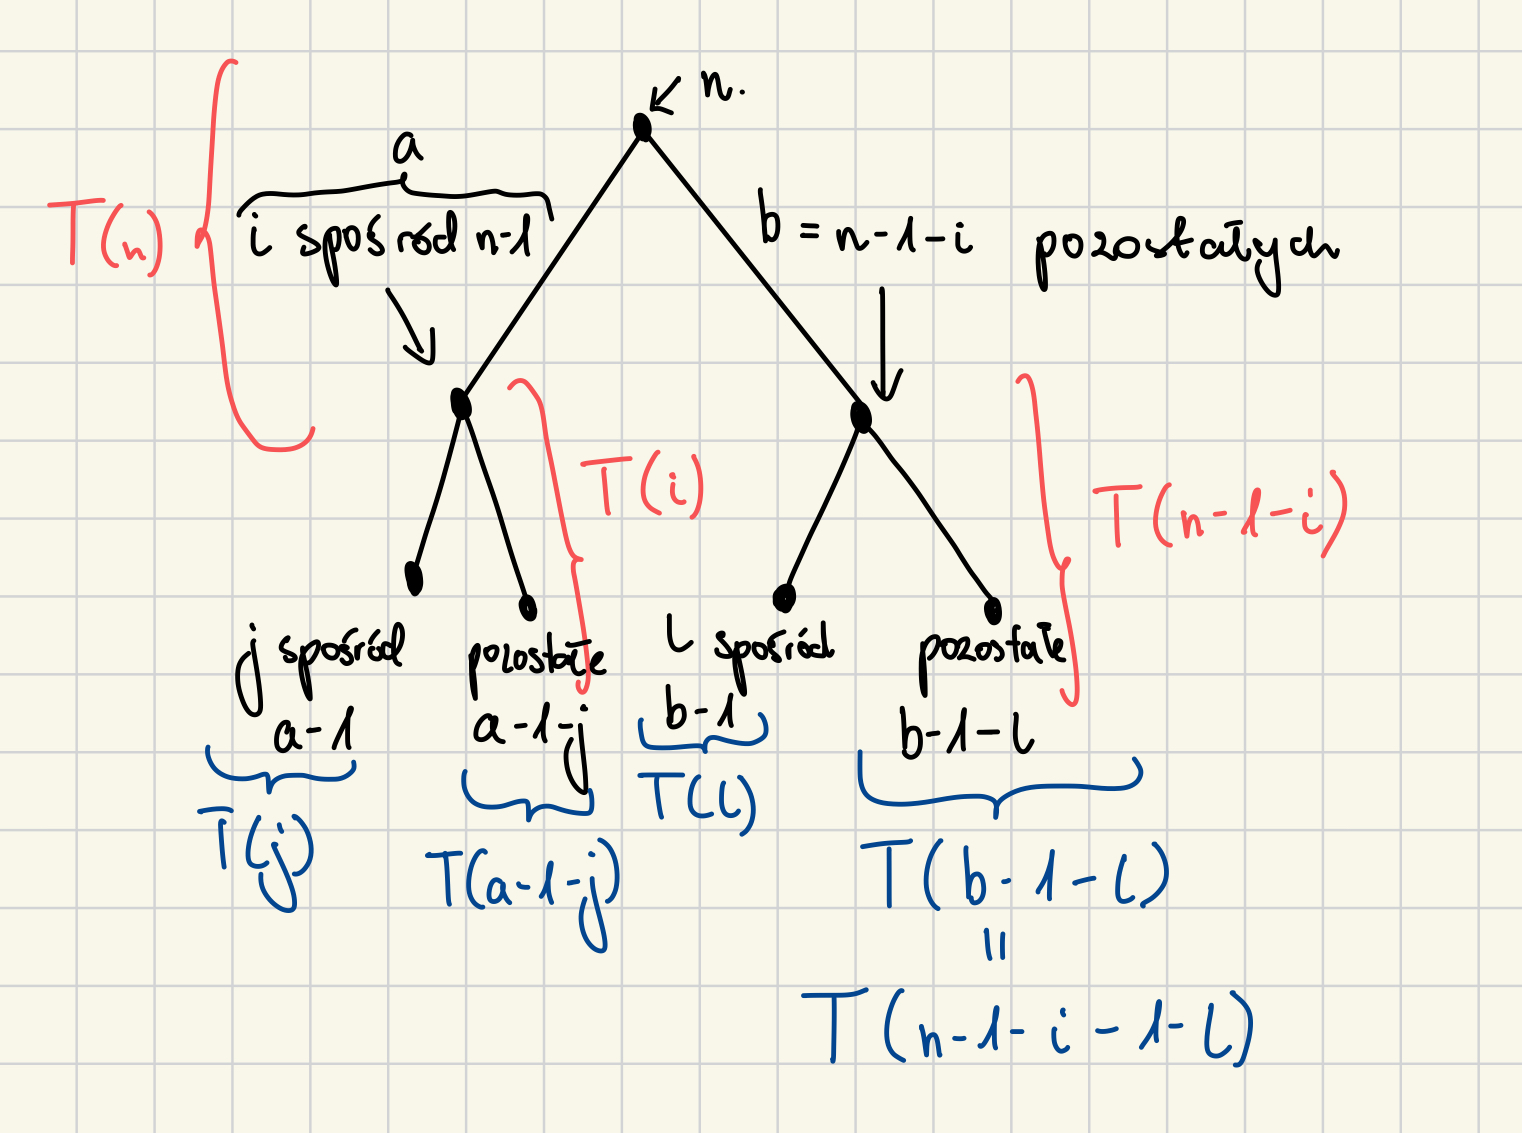
\includegraphics[width=0.7\textwidth]{images/zad36.jpeg}
    \end{center}

\end{mdframed}
\begin{mdframed}
    Rozwiązanie Autora 2.
\end{mdframed}




\begin{zad}[Mateusz Rabantek, Autor 2]
    Triangulacją $n$ -- wierzchołkowego wielokąta wypukłego nazywamy zbiór
    $(n - 3)$ wzajemnie nieprzecinających się jego przekątnych, które dzielą jego obszar na
    $(n - 2)$ trójkątów.
    \begin{enumerate}
        \item ile jest triangulacji $n$--wierzchołkowego wielokąta wypukłego?
        \item Ile jest triangulacji $n$--wierzchołkowego wielokąta wypukłego, w których każdy trójkąt
              triangulacji ma przynajmniej jeden bok na brzegu wielokąta?
    \end{enumerate}
\end{zad}
\begin{mdframed}
    \begin{enumerate}
        %rozwiązanie: Mateusz Rabantek
        \textbf{Podpunkt 1:}\newline
        $n+2$ wierzchołków\newline
        $T_{n+2}$ - triangulacje z krawędzią kończącą się w 1. Weźmy bok 12 - jest on częścią pewnego trójkąta $12i$. Jeśli $T_{n+2}$ = wszystkie triangulacje, 
        $T_{n+2}^{i}$ = te triangulacje z $T_n+2$, które zawierają trójkąt 12i. Stąd ${T_{n+2}^{i}}$ są parami rozłączne oraz $T_{n+2}$ = $\bigcup_{i=3}^{n+2} T_{n+2}^{i}$
        \newline
        Mamy: 
        \[|T_{n+2}| = 
        \sum_{i=3}^{n+2} |T_{n+2}^{i}| = \sum_{i=3}^{n+2} \left( |T_{i-1}| \cdot |T_{n+3-i}| \right)
        \]
        $|T_2|$ = 1, $|T_3|$ = 1. Otrzymujemy rekurencje dla liczb Catalana z przesuniętymi indeksami.
        \newline
        \newline
        \textbf{Podpunkt 2:}\newline
        $n$ wierzchołków\newline
        Wybierzmy bok 12 i zauważmy, że 12 jest częscią pewnego trójkąta 12i.\newline
        \textbf{i = 3,n:}\newline
             Zauważmy, że w przypadku $i = 3$, krawędź musi być częscią trójkąta 134 lub 13n. Stąd liczba triangulacji $2^{n-4}$ (analogicznie dla i=n)
        \newline
        \textbf{i $\neq$ 3, i $\neq$ n}\newline
            Wybieramy lewa/prawa strone: $2^{i-4}$ $\cdot$ $2^{n-i-1}$ = $2^{n-5}$\newline
        \textbf{Wynik:} $2^{n-4}$ + $2^{n-4}$ + $(n-4)$ $\cdot$ $2^{n-5}$ = $n2^{n-5}$


    \end{enumerate}
\end{mdframed}
\begin{mdframed}
    \begin{enumerate}
        \item Rozwiązanie Autora 2 podpunktu 1
        \item Rozwiązanie Autora 2 podpunktu 2
    \end{enumerate}
\end{mdframed}




\begin{zad}[Autor 1, Autor 2]
    Wykaż, że liczba drzew etykietowanych na zbiorze ${1, ..., n}$ wynosi $n^{n-2}$.
\end{zad}
\begin{mdframed}
    Rozwiązanie Autora 1.
\end{mdframed}
\begin{mdframed}
    Rozwiązanie Autora 2.
\end{mdframed}























\newpage
\section{Zestaw}          % ZESTAW 4

\begin{zad}[Julian Sowiński, Autor 2]
    Oblicz $S(n, 2)$.
\end{zad}
\begin{mdframed}
    Liczba Stirlinga drugiego rodzaju $S(n, k)$ dla $k=2$ to tak właściwie liczba sposobów na podzielenie zbioru $n$-elementowego na 2 niepuste podzbiory.
    $$S(n, 2) = \frac{\overbrace{2^n}^{\text{wszystkie podzbiory}} - \overbrace{2}^{\text{bez pustego i całego}}}{\underbrace{2}_{\text{nie bierzemy pod uwagę kolejności}}} = \frac{2^n - 2}{2} = 2^{n-1} - 1$$
\end{mdframed}
\begin{mdframed}
    Rozwiązanie Autora 2.
\end{mdframed}




\begin{zad}[Autor 1, Krzysztof Wójtowicz]
    Wykaż, że mamy dokładnie
    \[\frac{n!}{1^{\lambda_1} \cdot 2^{\lambda_2} \cdot  ... \cdot n^{\lambda_n} \cdot \lambda_1! \cdot ... \cdot \lambda_n!}\]
    permutacji zbioru $[n]$ o typie $1^{\lambda_1} \cdot 2^{\lambda_2} \cdot ... \cdot n^{\lambda_n} $  (mających $\lambda_i$ cykli długości i dla $i \in [n]$).
\end{zad}
\begin{mdframed}
    Rozwiązanie Autora 1.
\end{mdframed}
\begin{mdframed}
    Niech $A$ będzie zbiorem wszystkich permutacji zbioru $[n]$ o typie jak w poleceniu.
    Niech $a_i \in [n]$, policzymy ilość cykli długości $k$: $(a_1,a_2,\ldots,a_k)$ w zbiorze $n$ elementowych:
    \[\binom{n}{k} \cdot \frac{k!}{k} = \frac{n!}{(n-k)! \cdot k}\]
    Wybieramy $k$ elementów do cyklu i następnie wybieramy ich kolejność (pierwszy element
    nie ma znaczenia w cyklu), stąd powyższy wynik.
    \newline \newline
    Policzymy ilość wszystkich możliwych cykli długości $1,2,\ldots,n$:
    \[\underbrace{\frac{n!}{(n-1)! \cdot 1} \cdot \frac{(n-1)!}{(n-2)! \cdot 1} \cdot \ldots}_{\lambda_1} \cdot
        \underbrace{\frac{(n-\lambda_1)!}{(n-\lambda_1-2)! \cdot 2} \cdot \ldots}_{\lambda_2} \cdot \ldots =
        \frac{n!}{1^{\lambda_1} \cdot 2^{\lambda_2} \cdot \ldots \cdot n^{\lambda_n}} \]
    Czyli mnożymy ilość możliwych cykli $k$ elementowych dla $\lambda_k$ ich ilości.
    \newline \newline
    W celu otrzymania liczby $|A|$ musimy jeszcze uzwględnić brak znaczenia kolejności
    występowania cykli w permutacji, liczba możliwych ustawień to:
    \[{\lambda_1}! \cdot {\lambda_2}! \cdot \ldots \cdot {\lambda_n}!\]
    Zatem liczba wszystkich permutacji $a \in A$:
    \[|A| = \frac{n!}{1^{\lambda_1} \cdot 2^{\lambda_2} \cdot \ldots \cdot n^{\lambda_n}
            \cdot {\lambda_1}! \cdot {\lambda_2}! \cdot \ldots \cdot {\lambda_n}!} \; \; \; \; \blacksquare\]
\end{mdframed}




\begin{zad}[Maciej Wełpa, Autor 2]
    Posługując się interpretacją kombinatoryczną, wykaż tożsamość:
    \[S(n+1,m+1) = \sum_k \binom{n}{k}S(k,m)\]
\end{zad}
\begin{mdframed}
    % Rozwiązanie: Maciej Wełpa
    \textbf{Lewa strona:} Podział zbioru n+1-elementowego na m+1 niepustych podzbiorów\\
    \textbf{Prawa strona:} Bierzemy n+1 element i tworzymy z niego nowy zbiór (domyślnie podzbiór nr m+1). Z pozostałych
    n elementów wybieramy n-k (\(\binom{n}{k}\) =\(\binom{n}{n-k}\)), które będą w zbiorze nr m+1 z elementem n+1. Pozostałe k elementów dzielimy na m niepustych podzbiorów. Używamy sumy, aby rozważyć wszystkie możliwości podzielenia elementów.
\end{mdframed}
\begin{mdframed}
    Rozwiązanie Autora 2.
\end{mdframed}




\begin{zad}[Autor 1, Autor 2]
    Zakładając, że zachodzi równość:
    \[
        (x_1 + ... + x_k)^n = \sum_{n_1+...+n_k=n}\binom{n}{n_1 n_2 ... n_k}x_1^{n_1}\cdot...\cdot x_k^{n_k}
    \]
    podaj ile wynosi $\binom{n}{n_1 n_2 ... n_k}$.
\end{zad}
\begin{mdframed}
    Rozwiązanie Autora 1.
\end{mdframed}
\begin{mdframed}
    Rozwiązanie Autora 2.
\end{mdframed}




\begin{zad}[Katarzyna Szwed, Autor 2]
    Wykaż, że
    \[
        \sum_{i=0}^{n} i \left[ n \atop i \right] = n! H_n,
    \]
    gdzie $H_n = 1 + \frac{1}{2} + ... + \frac{1}{n}$.
\end{zad}
\begin{mdframed}
    %Rozwiązanie: Katarzyna Szwed
    Rozważmy zbiór $X := \{(\sigma, c) : \sigma$ - permutacja zbioru $[n]$, $c$ - wyróżniony cykl z permutacji $\sigma\}$.

    Rozważmy rodzinę zbiorów $\{A_i\}_{i=0}^{n}$ taką, że $A_i = \{(\sigma, c) \in X :$ permutacja $\sigma$ ma $i$ cykli$\}$.
    Zauważmy, że $|A_i| = i\left[ n \atop i\right]$ (najpierw liczymy liczbę permutacji $[n]$ o $i$ cyklach, a potem wybieramy
    jeden z $i$ cykli).

    Rodzina $A_i$ jest rozłącznym pokryciem zbioru $X$, zatem:
    \[|X| = \sum_{i=0}^{n} |A_i| = \sum_{i=0}^{n} i\left[ n \atop i\right]\].

    Teraz rozważmy rodzinę zbiorów $\{B_k\}_{k=1}^{n}$ taką, że $B_k = \{(\sigma, c) \in X :$ cykl $c$ ma $k$ elementów$\}$.
    Zauważmy, że $|B_k| = {n \choose k} \frac{k!}{k} (n-k)!$, ponieważ najpierw wybieramy $k$ elementów do cyklu $c$, potem permutujemy
    je, ale usuwamy kolejność pierwszego elementu, na koniec permutujemy resztę elementów zbioru $[n]$.

    Rodzina $B_k$ jest rozłącznym pokryciem zbioru $X$, zatem:
    \[
        |X| = \sum_{k=1}^{n} |B_k| = \sum_{k=1}^{n} {n \choose k} \frac{k!}{k} (n-k)! = \\
        \sum_{k=1}^n \frac{n!}{k!(n-k)!}\frac{k!}{k} (n-k)! = \sum_{k=1}^{n}\frac{n!}{k} =
        n! \sum_{k=1}^{n} \frac{1}{k} = n! H_n
    \]

    Otrzymujemy więc:
    \[\sum_{i=0}^{n} i\left[ n \atop i\right] = n! H_n\]


\end{mdframed}
\begin{mdframed}
    Rozwiązanie Autora 2.
\end{mdframed}




\begin{zad}[Julian Sowiński, Autor 2]
    Wykaż, że dla dowolnego $x \in \mathbb{R}$ zachodzi:
    \begin{enumerate}
        \item $x^n = \sum_{k}S(n,k) x^{\underline{k}}$
        \item $x^{\bar{n}} = \sum_{k} \left[n \atop k \right] x^k$.
    \end{enumerate}
\end{zad}
\begin{mdframed}
    \begin{enumerate}
        \item
              $$x^n = \sum_{k=0}^n S(n,k) x^{\underline{k}}$$
              Dowód indukcyjny:
              \newline \newline
              1) Dla $n=0$: \\
              L = $x^{\underline{0}} = 1$ \\
              P = $S(0,0) \cdot x^{\underline{0}} = 1 \cdot 1 = 1$ \\
              L = P

              2) Dla $n>0$:

              Założenie: $$x^n = \sum_{k=0}^n S(n,k) x^{\underline{k}}$$

              Teza: $$x^{n+1} = \sum_{k=0}^{n+1} S(n+1,k) x^{\underline{k}}$$

              Rozpoczynamy od lewej strony, używając założenia indukcyjnego:
              $$L = x \cdot x^n = x \cdot \sum_{k=0}^n S(n,k) x^{\underline{k}} = \sum_{k=0}^n S(n,k) (x \cdot x^{\underline{k}}) \quad (*)$$

              Zauważmy, że:
              \begin{align*}
                  \cdot x^{\underline{k}}*x & = (x-k+k) x^{\underline{k}} = (x-k) x^{\underline{k}} + k x^{\underline{k}} = x^{\underline{k+1}} + k x^{\underline{k}}
              \end{align*}

              Kontynuujemy z (*), podstawiając znalezioną tożsamość:
              \begin{align*}
                  (*) & = \sum_{k=0}^n S(n,k) (x^{\underline{k+1}} + k x^{\underline{k}})                   \\
                      & = \sum_{k=0}^n S(n,k) x^{\underline{k+1}} + \sum_{k=0}^n k S(n,k) x^{\underline{k}}
              \end{align*}

              Teraz zmienimy przedziały sumowania:
              \begin{align*}
                  \star & = \sum_{k=1}^{n+1} S(n,k-1) x^{\underline{k}} + \underbrace{\sum_{k=0}^{n+1} k S(n,k) x^{\underline{k}}}_{\text{ponieważ } S(n,n+1)=0} \\
                        & = \underbrace{\sum_{k=0}^{n+1} S(n,k-1) x^{\underline{k}}}_{\text{ponieważ } S(n,-1)=0} + \sum_{k=0}^{n+1} k S(n,k) x^{\underline{k}}  \\
                        & = \sum_{k=0}^{n+1} (S(n,k-1) + k S(n,k)) x^{\underline{k}}                                                                             \\
                        & = \sum_{k=0}^{n+1} S(n+1,k) x^{\underline{k}} = P
              \end{align*}

              Co dowodzi tezy indukcyjnej.
              \newline

        \item $$x^{\bar{n}} = \sum_{k} \left[n \atop k \right] x^k$$

              Dowód indukcyjny:

              1) Dla $n=0$:
              \newline
              L = $x^{\overline{0}} = 1$
              \newline
              P = $\sum_{k=0}^0 \genfrac{[}{]}{0pt}{1}{0}{k} x^k = \genfrac{[}{]}{0pt}{1}{0}{0} x^0 = 1 \cdot 1 = 1$.
              \newline
              L = P
              \newline

              2) Dla $n>0$:
              \newline
              Założenie:
              $$x^{\overline{n-1}} = \sum_{k=0}^{n-1} \genfrac{[}{]}{0pt}{1}{n-1}{k} x^k$$

              Teza:
              $$x^{\overline{n}} = \sum_{k=0}^n \genfrac{[}{]}{0pt}{1}{n}{k} x^k$$
              Rozpoczynamy od lewej strony:
              \begin{align*}
                  L & = x^{\overline{n}} = (x+n-1) x^{\overline{n-1}} = (x+n-1) \sum_{k=0}^{n-1} \genfrac{[}{]}{0pt}{1}{n-1}{k} x^k                   \\
                    & = \sum_{k=0}^{n-1} (x+n-1) \genfrac{[}{]}{0pt}{1}{n-1}{k} x^k                                                                   \\
                    & = \sum_{k=0}^{n-1} \genfrac{[}{]}{0pt}{1}{n-1}{k} x^{k+1} + \sum_{k=0}^{n-1} (n-1) \genfrac{[}{]}{0pt}{1}{n-1}{k} x^k \quad (*)
              \end{align*}

              Teraz zmieniamy przedziały sumowania, aby później zastosować wzór rekurencyjny:

              \begin{align*}
                  (*) & = \sum_{k=0}^{n} \genfrac{[}{]}{0pt}{1}{n-1}{k-1} x^k + \sum_{k=0}^{n} (n-1) \genfrac{[}{]}{0pt}{1}{n-1}{k} x^k \\
                      & = \sum_{k=0}^{n} \left(\genfrac{[}{]}{0pt}{1}{n-1}{k-1} + (n-1) \genfrac{[}{]}{0pt}{1}{n-1}{k}\right) x^k
              \end{align*}
              Stosujemy wzór rekurencyjny dla liczb Stirlinga I rodzaju:
              $$\genfrac{[}{]}{0pt}{1}{n}{k} = (n-1)\genfrac{[}{]}{0pt}{1}{n-1}{k} + \genfrac{[}{]}{0pt}{1}{n-1}{k-1}$$
              Podstawiając to do naszego wyrażenia, otrzymujemy:
              \begin{align*}
                   & = \sum_{k=0}^{n} \genfrac{[}{]}{0pt}{1}{n}{k} x^k = P
              \end{align*}
              Co kończy dowód indukcyjny.
    \end{enumerate}
\end{mdframed}
\begin{mdframed}
    \begin{enumerate}
        \item Rozwiązanie Autora 2 podpunktu 1
        \item Rozwiązanie Autora 2 podpunktu 2
    \end{enumerate}
\end{mdframed}















\newpage
\section{Zestaw}          % ZESTAW 5

\begin{zad}[Autor 1, Autor 2]
    Wykaż zasadę włączeń i wyłączeń korzystając z indukcji po liczbie zbiorów.
\end{zad}
\begin{mdframed}
    Rozwiązanie Autora 1.
\end{mdframed}
\begin{mdframed}
    Rozwiązanie Autora 2.
\end{mdframed}




\begin{zad}[Autor 1, Autor 2]
    Wykaż, że mamy
    \[
        \sum_{j=0}^{m}(-1)^j \binom{m}{j}(m-j)^n
    \]
    suriekcji ze zbioru $[n]$ w zbiór $[m]$.
\end{zad}
\begin{mdframed}
    Rozwiązanie Autora 1.
\end{mdframed}
\begin{mdframed}
    Rozwiązanie Autora 2.
\end{mdframed}



\begin{zad}[Bartosz Wójcik, Autor 2]
    Ile jest ciągów długości $2n$ takich, że każda liczba $i \in [n]$
    występuje dokładnie dwa razy oraz każde sąsiednie dwa wyrazy są różne.
\end{zad}

\begin{mdframed}
    % Rozwiązanie: Bartosz Wójcik

    Niech $\Omega$ będzie zbiorem ciągów długości $2n$, że każda liczba $i \in [n]$
    występuje dokładnie dwa razy.
    Niech $X \subseteq \Omega$ będzie zbiorem ciągów, w których żadne sąsiadujące wyrazy
    nie są równe (zbiór jak w treści zadania).
    Niech $A_i \subseteq \Omega$, będzie rodziną zbiorów,
    takich że:

    $$ A_i = \{a \in X \vert\text{ liczba i sąsiaduje ze sobą w ciągu a }\} $$

    Zbiór $X$ zawiera wszystkie ciągi, które należą do $\Omega$, ale nie należą do żadnego
    $A_i$:

    $$ X = \Omega \setminus \bigcup_{i = 1}^{n} A_i$$

    Obliczmy moc sumy $A_i$:

    $$ (*) \
        |\bigcup_{i = 1}^{n} A_i| = \sum_{\emptyset\neq I \subseteq [n]} (-1)^{|I| + 1} \
        |\bigcap_{i \in I} A_i|
    $$

    Wybierzmy ciąg $a \in \bigcap_{i \in I} A_i$. Wszystkie $i \in I$ sąsiadują ze sobą,
    więc można je potraktować jako jeden znak. W ciągu $a$ mamy więc $2n - |I|$ znaków,
    które można przepermutować na $(2n - |I|)!$ sposobów. Każdą parę $\notin I$ można ustawić na 2
    sposoby każdą. Sumarycznie:
    $$\
        |\bigcap_{i \in I} A_i| = \frac{(2n - |I|)!}{2^{n - |I|}}\
    $$

    Zmieńmy indeksowanie sumy $(*)$ z indeksowania po zbiorach $I$ na indeksowanie po mocy zbioru $I$.
    Jest $\binom{n}{i}$ zbiorów $I \subseteq [n], |I| = i$:

    $$(*)\
        \sum_{\emptyset\neq I \subseteq [n]} (-1)^{|I| + 1} \
        |\bigcap_{i \in I} A_i| = \
        \sum_{i = 1}^{n} (-1)^{i + 1} \binom{n}{i} \frac{(2n - i)!}{2^{n - i}}\
    $$

    Dodatkowo $|\Omega| = \frac{(2n)!}{2^{n}}$. Otrzymujemy:

    $$(*)\
        |X| = \frac{(2n)!}{2^{n}} - \sum_{i = 1}^{n} (-1)^{i + 1} \binom{n}{i} \frac{(2n - i)!}{2^{n - i}} = \
        \sum_{i = 0}^{n} (-1)^{i} \binom{n}{i} \frac{(2n - i)!}{2^{n - i}} \
    $$
    co było do policzenia. $\blacksquare$


\end{mdframed}

\begin{mdframed}
    Rozwiązanie Autora 2.
\end{mdframed}




\begin{zad}[Karol Wójcik, Autor 2]
    Wykaż, że dla $n \geq 3$ zachodzi tożsamość
    \[
        D(n) = (n-1)(D(n-1) + D(n-2))
    \]
    gdzie $D(n)$ jest liczbą permutacji zboru $[n]$ bez punktów stałych.
\end{zad}
\begin{mdframed}
    % Rozwiązanie: Karol Wójcik
    Dla $n \ge 3$:   $D(n) = (n-1)(D(n-1)+D(n-2))$
    \newline \newline
    D(n) - liczba nieporządków
    \newline \newline
    $D(1) = 0$      $D(2) = 1$
    \newline \newline
    $D_n$ -- zbiór nieporządków na $n$ elementach
    \newline \newline
    Weźmy zbiór $D_n = X \cup Y$, $X \cap Y = \emptyset$.

    $X$ -- zbiór, gdzie $n$ znajduje się w 2-elementowym cyklu,

    $Y$ -- zbiór, gdzie $n$ znajduje się w $>$ 2-elementowym cyklu
    \newline \newline
    $X = \{ (i,n) \ast \sigma \mid \sigma \text{ jest permutacją na } [n] \setminus \{i,n\} \text{ bez punktów stałych, } i \in [n-1] \}$

    $|X| = \lvert [n-1] \rvert \cdot \lvert D(n-2) \rvert = (n-1)D(n-2)$
    \newline \newline
    $Y = \{ \sigma \mid \sigma(j)=n, \sigma(n)=i, i \neq j \}$

    $|Y| = (n-1)D(n-1)$
    \newline \newline
    $D(n) = |X \cup Y| = (n-1)(D(n-1) + D(n-2))$
\end{mdframed}
\begin{mdframed}
    Rozwiązanie Autora 2.
\end{mdframed}




\begin{zad}[Autor 1, Autor 2]
    Wykaż (najlepiej kombinatorycznie), że dla dowolnych $n, k \in \mathbb{N}$
    zachodzi:
    \begin{enumerate}
        \item $S(n, k) = \sum_{0 \leq m_1 \leq m_2 \leq ... \leq m_{n-k} \leq k} m_1m_2 \cdot ... \cdot m_{n-k}$
        \item $c(n, k) = \sum_{0 < m_1 < m_2 < ... < m_{n-k} < k} m_1m_2 \cdot ... \cdot m_{n-k}$
    \end{enumerate}
\end{zad}
\begin{mdframed}
    \begin{enumerate}
        \item Rozwiązanie Autora 1 podpunktu 1
        \item Rozwiązanie Autora 1 podpunktu 2
    \end{enumerate}
\end{mdframed}
\begin{mdframed}
    \begin{enumerate}
        \item Rozwiązanie Autora 2 podpunktu 1
        \item Rozwiązanie Autora 2 podpunktu 2
    \end{enumerate}
\end{mdframed}


\begin{zad}[Autor 1, Autor 2]
    Ciąg podziałów zbioru ${1, ..., n}$ tworzymy następująco. Startujemy
    od podziału zawierającego tylko zbiór ${1, ..., n}$. Podział $(i + 1)$--wszy
    otrzymujemy z podziału $i$-tego poprzez:
    \begin{enumerate}
        \item wybranie jednego, co najmniej $2$-elementowego zbioru z podziału $i$-tego i podzielenie
              go na dwa niepuste podzbiory,
        \item podzielenie każdego, co najmniej $2$-elementowego zbioru z podziału $i$-tego na dwa
              niepuste podzbiory.
    \end{enumerate}
    W obu przypadkach procedura kończy swoje działanie jeżeli wszystkie zbiory podziału są
    jednoelementowe. Na ile sposobów można wykonać powyższe procedury? Na ile sposobów
    możemy wykonać powyższe procedury zakładając, że po każdym kroku zbiory podziałów
    zawierają kolejne liczby naturalne?
\end{zad}
\begin{mdframed}
    Rozwiązanie Autora 1.
\end{mdframed}
\begin{mdframed}
    Rozwiązanie Autora 2.
\end{mdframed}


\newpage
\section{Zestaw 6}          % Zestaw 6

\begin{zad}(nie kolos)
    Wykaż, że spośród dowolnych trzech permutacji zbioru $[n]$
    istnieją dwie zawierające wspólny podciąg o długości co najmniej $n^{\frac{1}{3}}$.
\end{zad}
\begin{mdframed}

\end{mdframed}
\begin{mdframed}

\end{mdframed}


\begin{zad}(kolos)
    Niech $I$ będzie rodziną $n$ przedziałów osi rzeczywistej.
    Wykaż, że $I$ zawiera co najmniej $\sqrt{n}$ przedziałów
    parami rozłącznych lub $I$ zawiera co najmniej $\sqrt{n}$
    przedziałów takich, że wszystkie posiadają wspólny punkt.

    Rodzina podzbiorów $\mathcal{F}$ jest przecinająca się, jeśli
    dla dowolnych $A, B \in \mathcal{F}$ mamy $A \cap B \neq \emptyset$
\end{zad}
\begin{mdframed}

\end{mdframed}
\begin{mdframed}

\end{mdframed}


\begin{zad}(kolos)
    Niech $\mathcal{F}$ będzie maksymalną przecinającą się rodziną podzbiorów $[n]$.
    Wykaż, że:
    \[ |\mathcal{F}| = 2^{n-1} \]
\end{zad}
\begin{mdframed}

\end{mdframed}
\begin{mdframed}

\end{mdframed}



\begin{zad}(kolos)
    Niech $\mathcal{F}$ będzie maksymalną rodziną podzbiorów zbioru $[n]$ taką,
    że dla dowolnych $A, B \in \mathcal{F}$ mamy $A \cup B \neq [n]$. Wyznacz $|\mathcal{F}|$.
\end{zad}
\begin{mdframed}

\end{mdframed}
\begin{mdframed}

\end{mdframed}


\begin{zad}
    Rodzina podzbiorów $\mathcal{F}$ zbioru $[n]$ jest rozróżniająca jeśli dla dowolnych
    $x \neq y \in [n]$ istnieje $F \in \mathcal{F }$ taki, że $|F \cap \{x,y\}| = 1$.
    Rodzina podzbiorów $\mathcal{F }$ zbioru $[n]$ jest silenie rozróżniająca jeśli dla
    dowolnych $ x \neq y \in [n]$ istnieje $F_1,F_2 \in \mathcal{F }$ takie, że $x \in F_1-F_2$ i $y \in F_2 - F_1$.
    \begin{enumerate}
        \item Jaki jest rozmiar najmniejszej rodziny rozróżniającej $[n]$?
        \item Jaki jest rozmiar najmniejszej rodziny silnie rozróżniającej $[n]$?
    \end{enumerate}
\end{zad}
\begin{mdframed}

\end{mdframed}
\begin{mdframed}

\end{mdframed}


\begin{zad}
    Niech $1 \leq s < r < n$ i niech $\mathcal{F }$ będzie rodziną podzbiorów $r$--elementowych
    zbioru $[n]$ taką, że dla dowolnych $A \neq B \in \mathcal{F }$ mamy $ |A \cap B| \leq s$.
    Wykaż, że \[|\mathcal{F }| \leq \frac{\binom{n}{s+1}}{\binom{r}{s+1}}.\]
\end{zad}
\begin{mdframed}

\end{mdframed}
\begin{mdframed}

\end{mdframed}













\newpage
\section{Zestaw 7}          % Zestaw 7
% Nothing here. Tylko work in progress...
Nie ma XD

Ponoć Profesor coś zakręcił i nie ma tego zestawu.































\newpage
\section{Zestaw}          % Zestaw 8

\begin{zad}[Krzysztof Wójtowicz, Autor 2]
    Wykorzystaj funkcje tworzące aby policzyć na ile sposobów można wyciągnąć 70 kul z urny zawierającej 30 kul czerwonych, 40 kul niebieskich i 50 kul białych. Kule tego samego koloru są nierozróżnialne. Kolejność wyciągania jest nieistotna.
\end{zad}
\begin{mdframed}
    Zapiszemy funkcje tworzące $C(x)$, $N(x)$ oraz $B(x)$ odpowiednio dla kul czerwonych(1), niebieskich(2) oraz białych(3):
    \begin{align}
        C(x) = 1 + x + x^2 + \dots + x^{30} = \frac{1 - x^{31}}{1 - x} \\
        N(x) = 1 + x + x^2 + \dots + x^{40} = \frac{1 - x^{41}}{1 - x} \\
        B(x) = 1 + x + x^2 + \dots + x^{50} = \frac{1 - x^{51}}{1 - x}
    \end{align}
    Stworzymy funkcję $K(x)$, która będzie generować nam ciąg liczby sposóbów wyciągania danej ilości kul, odpowiedzią dla 70 kul będzie współczynnik przy $x^{70}$.
    \begin{gather*}
        K(x) = C(x) \cdot N(x) \cdot B(x) = \frac{(1 - x^{31})(1 - x^{41})(1 - x^{51})}{(1 - x)^3} = \\
        = (1 - x^{31} - x^{41} - x^{51} + x^{72} + x^{82} + x^{92} - x^{123}) \cdot \sum_{k=0}^{\infty} \binom{k+2}{2}x^k
    \end{gather*}
    Po wymnożeniu $x^{70}$ wystąpi cztery razy:
    \begin{enumerate}
        \item dla $k = 70$: \[ 1 \cdot \binom{72}{2}x^{70} = \binom{72}{2}x^{70}\]
        \item dla $k = 39$: \[ -x^{31} \cdot \binom{41}{2}x^{39} = -\binom{41}{2}x^{70}\]
        \item dla $k = 29$: \[ -x^{41} \cdot \binom{31}{2}x^{29} = -\binom{31}{2}x^{70}\]
        \item dla $k = 19$: \[ -x^{51} \cdot \binom{21}{2}x^{19} = -\binom{21}{2}x^{70}\]
    \end{enumerate}
    Więc współczynnik przy $x^{70}$ wynosi:
    \begin{gather*}
        \binom{72}{2} - \binom{41}{2} - \binom{31}{2} - \binom{21}{2} = \frac{72!}{2! \cdot 70!} - \frac{41!}{2! \cdot 39!} - \frac{31!}{2! \cdot 29!} - \frac{21!}{2! \cdot 19!} = \\ = 2556 - 820 - 465 - 210 = 1061
    \end{gather*}

\end{mdframed}
\begin{mdframed}
    Rozwiązanie Autora 2.
\end{mdframed}

\begin{zad}[Krzysztof Wójtowicz, Autor 2]
    Jaki jest współczynnik
    \begin{enumerate}
        \item przy $x^5$ w $(1-2x)^{-2}$;
        \item przy $x^4$ w $\sqrt[3]{1+x}$;
        \item przy $x^3$ w $(2+x)^{3/2}/(1-x)$?
    \end{enumerate}
\end{zad}
\begin{mdframed}
    \textbf{Podpunkt 1.} \newline
    Niech:
    \[ F(x) = \frac{1}{2} \cdot \frac{1}{1-2x} = \frac{1}{2} \cdot \sum_{n=0}^{\infty} (2x)^n \]
    Wtedy:
    \begin{gather*}
        F'(x) = \frac{1}{(1-2x)^2} = (1-2x)^{-2} = \frac{1}{2} \cdot \sum_{n=1}^{\infty} (2^n \cdot n \cdot x^{n-1}) = \\ = \sum_{n=0}^{\infty} (\underbrace{2^n \cdot (n+1)}_{a_n} \cdot x^n)
    \end{gather*}
    Więc:
    \[ a_5 = 2^5 \cdot 6 = 192 \]
    \textbf{Podpunkt 2.} \newline
    Użyjemy rozwinięcia binomial series:
    \[ (1+x)^{1/3} = \sum_{n=0}^{\infty} \underbrace{\binom{\frac{1}{3}}{n}}_{a_n} \cdot x^n \]
    Więc:
    \[ a_4 = \binom{\frac{1}{3}}{4} = \frac{\frac{1}{3}(\frac{1}{3} - 1)(\frac{1}{3} - 2)(\frac{1}{3} - 3)}{4!} = \frac{-10}{243} \]
    \textbf{Podpunkt 3.} \newline
    Rozwiniemy osobno mianownik i licznik:
    \begin{gather*}
        (2+x)^{3/2} = 2^{3/2}(1+\frac{x}{2})^{3/2} = 2\sqrt{2} \cdot \sum_{n=0}^{\infty} \binom{\frac{3}{2}}{n}(\frac{x}{2})^n \\
        \frac{1}{1-x} = \sum_{n=0}^{\infty} x^n
    \end{gather*}
    Wtedy:
    \[ \frac{(2+x)^{3/2}}{1-x} = \sum_{n=0}^{\infty} c_n \cdot x^n \]
    Gdzie $c_n$ jest równe (iloczyn Cauchy'ego):
    \[ c_n = 2\sqrt{2} \cdot \sum_{k=0}^{n} \binom{\frac{3}{2}}{k} \cdot \frac{1}{2^k} \]
    Stąd otrzymujemy:
    \begin{gather*}
        c_3 = 2\sqrt{2} \cdot \sum_{k=0}^{3} \binom{\frac{3}{2}}{k} \frac{1}{2^k} = 2\sqrt{2}\cdot(1\cdot\binom{\frac{3}{2}}{0} + \frac{1}{2}\cdot\binom{\frac{3}{2}}{1} + \frac{1}{4}\cdot\binom{\frac{3}{2}}{2} + \frac{1}{8}\cdot\binom{\frac{3}{2}}{3}) = \\ = 2\sqrt{2} \cdot (1 + \frac{3}{4} + \frac{3}{32} - \frac{1}{128}) = 2\sqrt{2}\cdot\frac{235}{128} = \frac{235\sqrt{2}}{64}
    \end{gather*}
\end{mdframed}
\begin{mdframed}
    Rozwiązanie Autora 2.
\end{mdframed}

\begin{zad}[Filip Sajko]
    Wyznacz funkcje tworzące następujących ciągów. (Znajdź zwartą postać
    tych funkcji, to jest bez nieskończonych sum.)
    \begin{enumerate}
        \item$(0,0,0,0,-6,6,-6,6...)$
        \item$(1,0,1,0...)$
        \item $(1,2,1,4,1,8...)$
        \item $(\binom{c}{0}, \binom{c}{1}, \binom{c}{2}, ...)$
        \item $(1, \binom{c}{1}, \binom{c+1}{1}, \binom{c+2}{2}, ...)$
        \item $(1, c, c^2, ...)$
        \item $(1, \binom{m+1}{m}, \binom{m+2}{m},...)$
        \item $(0, 1, \frac{1}{2}, \frac{1}{3},...)$
        \item $(1, 1, \frac{1}{2!}, \frac{1}{3!},...)$
    \end{enumerate}
\end{zad}
\begin{mdframed}
    \begin{enumerate}

        \item$(0,0,0,0,-6,6,-6,6...)$
              \[-6x^4 + 6x^5 - 6x^6 + 6x^7 = \]

              \[ = -6x^4(1-x+x^2-x^3 + ...) = \frac{-6x^4+6x^5}{1-x^2} = \frac{-6x^4}{1+x} \]

        \item$(1,0,1,0...)$
              \[1+x^2+x^4+... = \frac{1}{1-x^2}\]

        \item $(1,2,1,4,1,8...)$
              \[1 + 2x + 1x^2 + 4x^3 + 1x^4 + 8x^5 + ... = (1 + x^2 + x^4 + x^6 +...) + (2x+4x^3+8x^5 + ...) = \frac{1}{1-x^2} + \frac{2x}{1-2x^2} \]

        \item $(\binom{c}{0}, \binom{c}{1}, \binom{c}{2}, ...)$
              \[1+ \binom{c}{1}+ \binom{c+1}{1}x+ \binom{c+2}{2}x^2 + ... = \sum_{n}^{}\binom{c}{n}x^n = (1+x)^c \]

        \item $(1, \binom{c}{1}, \binom{c+1}{1}, \binom{c+2}{2}, ...)$
              \[a_n = \binom{c+n-1}{n-1}\]
              \[1 + \sum_{n \geq 1}^{} \binom{c+n-1}{n-1}x^n = 1 + x \sum_{n-1 \leq 0 }^{}\binom{c+n-1}{n-1}x^{n-1} = 1 + \frac{1}{(1-x)^{c+1}}\]

        \item $(1, c, c^2, ...)$
              \[1+cx+c^2x^2+...=1+(cx)^2+(cx)^3+ ... = \frac{1}{1-cx}\]

        \item $(1, \binom{m+1}{m}, \binom{m+2}{m},...)$
              \[a_n = \binom{m+n}{m}  = \binom{n+m}{n} \]
              \[\sum_{}^{}a_nx^n = \sum \binom{m+n}{n}x^n = \frac{1}{(1-x)^{m+1}}\]

        \item $(0, 1, \frac{1}{2}, \frac{1}{3},...)$
              \[0+ 1+ \frac{1}{2}+ \frac{1}{3}+... = 1 + \sum_{n=1}^{}\frac{x^n}{n} = 1 - \ln (1-x)\]

        \item $(1, 1, \frac{1}{2!}, \frac{1}{3!},...)$
              \[1 + 1x+ \frac{1}{2!}x + ... = \sum_{}^{}\frac{x^n}{n!} = e^x\]
    \end{enumerate}
\end{mdframed}
\begin{mdframed}
    Rozwiązanie Autora 2.
\end{mdframed}

\begin{zad}[Filip Sajko, Julian Sowiński]
    Niech $G(z)$ będzie funkcją tworzącą ciągu $\{g_n\}_{n \geq 0}$.
    Jaki ciąg generuje funkcja $G(z) + G(-z)$, a jaki $G(z) - G(-z)$?
\end{zad}
\begin{mdframed}
    \[G( z) = g_0 + g_1x + g_2x^2 + g_3x^3  + ...\]
    \[G(-z) = g_0 - g_1x + g_2x^2  - g_3x^3 + ...\]
    Stąd, po prostu dodając i odejmując stronami otrzymujemy:
    \[G(z) + G(-z) = 2(g_0 + g_2x^2 + g_4x^4 + ...)\]
    \[G(z) - G(-z) = 2(g_1x + g_3x^3 + g_5x^5 + ...)\]
\end{mdframed}
\begin{mdframed}
    $$ G(z) = g_0 + g_1 z + g_2 z^2 + g_3 z^3 + g_4 z^4 + \dots $$
    
    \subsection*{a) Funkcja tworząca $G(z) + G(-z)$}
    
    Najpierw zapiszmy postać funkcji $G(-z)$, podstawiając $-z$ w miejsce $z$:
    $$ G(-z) = \sum_{n=0}^{\infty} g_n (-z)^n = g_0 - g_1 z + g_2 z^2 - g_3 z^3 + g_4 z^4 - \dots $$
    Teraz dodajmy obie funkcje stronami. Zauważmy, że wszystkie wyrazy z nieparzystymi potęgami $z$ się skrócą:
    $$ G(z) + G(-z) = (g_0 + g_1 z + g_2 z^2 + \dots) + (g_0 - g_1 z + g_2 z^2 - \dots) $$
    $$ G(z) + G(-z) = (g_0+g_0) + (g_1-g_1)z + (g_2+g_2)z^2 + (g_3-g_3)z^3 + \dots $$
    $$ G(z) + G(-z) = 2g_0 + 2g_2 z^2 + 2g_4 z^4 + \dots = 2(g_0 + g_2x^2 + g_4x^4 + ...)$$

    \subsection*{b) Funkcja tworząca $G(z) - G(-z)$}

    Postępujemy analogicznie, tym razem odejmując funkcje. W tym przypadku skrócą się wyrazy z parzystymi potęgami $z$:
    $$ G(z) - G(-z) = (g_0 + g_1 z + g_2 z^2 + \dots) - (g_0 - g_1 z + g_2 z^2 - \dots) $$
    $$ G(z) - G(-z) = (g_0-g_0) + (g_1-(-g_1))z + (g_2-g_2)z^2 + (g_3-(-g_3))z^3 + \dots $$
    $$ G(z) - G(-z) = 2g_1 z + 2g_3 z^3 + 2g_5 z^5 + \dots = 2(g_1x + g_3x^3 + g_5x^5 + ...)$$
\end{mdframed}




\begin{zad}[Maciej Wełpa, Autor 2]
    Niech $a_n$ będzie liczbą trójek $(i,j,k)$ liczb całkowitych takich, że $i \geqslant 0, j \geqslant 1, k \geqslant 1$ oraz $i + 3j + 3k = n$. Znajdź funkcję tworzącą ciągu $(a_0,a_1,\dots)$ i wyznacz wzór na $a_n$.
\end{zad}
\begin{mdframed}
    Równanie: $i+3j+3k=n$, gdzie $i \ge 0, j \ge 1, k \ge 1$.
    \newline
    Funkcja tworząca dla zmiennej $i$ (dla $i \ge 0$):
    $$I(x) = \sum_{a=0}^{\infty} x^a = 1 + x + x^2 + \dots = \frac{1}{1-x}$$
    Funkcja tworząca dla zmiennej $j$ (dla $j \ge 1$ i $3j$ w równaniu):
    $$J(x) = \sum_{b=1}^{\infty} x^{3b} = x^3 + x^6 + x^9 + \dots = x^3(1 + x^3 + x^6 + \dots) = x^3 \sum_{c=0}^{\infty} (x^3)^c = \frac{x^3}{1-x^3}$$
    Funkcja tworząca dla zmiennej $k$ (dla $k \ge 1$ i $3k$ w równaniu):
    $$K(x) = \sum_{d=1}^{\infty} x^{3d} = x^3 + x^6 + x^9 + \dots = \frac{x^3}{1-x^3}$$
    Funkcja tworząca $a(x)$ dla liczby rozwiązań równania $i+3j+3k=n$ jest iloczynem funkcji tworzących dla poszczególnych zmiennych:
    $$a(x) = I(x) \cdot J(x) \cdot K(x) = \frac{1}{1-x} \cdot \frac{x^3}{1-x^3} \cdot \frac{x^3}{1-x^3}$$
    Zatem:
    $$a(x) = \frac{x^6}{(1-x)(1-x^3)^2}$$
    Aby znaleźć współczynnik $a_n$ (liczbę rozwiązań), należy rozłożyć $a(x)$ na ułamki proste. Mianownik możemy zapisać jako:
    $(1-x)(1-x^3)^2 = (1-x) ( (1-x)(1+x+x^2) )^2 = (1-x) (1-x)^2 (1+x+x^2)^2 = (1-x)^3 (1+x+x^2)^2$
    Stąd:
    $$a(x) = \frac{x^6}{(1-x)^3 (1+x+x^2)^2}$$
    Rozkład na ułamki proste dla tego typu wyrażenia będzie zawierał składniki postaci:
    $$\frac{A}{1-x} + \frac{B}{(1-x)^2} + \frac{C}{(1-x)^3} + \frac{Dx+E}{1+x+x^2} + \frac{Fx+G}{(1+x+x^2)^2}$$
    Wyznaczenie stałych $A, B, C, D, E, F, G$ jest procesem arytmetycznym i czasochłonnym, wymagającym podstawiania wartości $x$ lub porównywania współczynników.
    Po wyznaczeniu tych stałych, każdy z ułamków prostych powinno przekształcić się z powrotem do szeregu potęgowego.
\end{mdframed}
\begin{mdframed}
    Rozwiązanie Autora 2.
\end{mdframed}

\begin{zad}[Krzysztof Wójtowicz, Autor 2]
    Ustal liczbę naturalną $r \geqslant 2$ i niech $a_n$ będzie liczbą $r$-tupli $(i_1,\dots,i_r)$ nieujemnych liczb całkowitych takich, że $i_1 + \dots + i_r = n$
    \begin{enumerate}
        \item Wyznacz funkcję tworzącą ciągu $(a_0,a_1,\dots)$
        \item Przy pomocy tej funkcji wyznacz wzór na $a_n$.
    \end{enumerate}
\end{zad}
\begin{mdframed}
    \textbf{Podpunkt 1.} \newline
    Funkcja tworzącą ciągu $(a_0,a_1,\dots)$:
    \begin{gather*}
        A(x) = (1 + x + x^2 + \dots)^r = (\frac{1}{1-x})^r = \frac{1}{(1-x)^r} = \sum_{n=0}^{\infty} \underbrace{\binom{n+r-1}{n}}_{a_n} x^n
    \end{gather*}
    \textbf{Podpunkt 2.} \newline
    Wzór na $a_n$:
    \[ a_n = \binom{n+r-1}{n} \]
\end{mdframed}
\begin{mdframed}
    Rozwiązanie Autora 2.
\end{mdframed}

\begin{zad}[Maciej Wełpa (i), Autor 2]
    Niech $a(x)$ będzie funkcją tworzącą ciągu $(a_0,a_1,\dots)$. Wytłumacz dlaczego $a(x) \cdot \frac{1}{1-x}$ jest funkcją tworzącą $(a_0,a_0+a_1,a_0+a_1+a_2,\dots)$. Korzystając z tej obserwacji wyznacz wzór zwarty na:
    \begin{enumerate}
        \item $\sum_{k=1}^{n} k^2$
        \item $\sum_{k=1}^{n} k^3$
    \end{enumerate}
\end{zad}
\begin{mdframed}
    \textbf{Wyjaśnienie właściwości funkcji tworzącej:} \newline
    Niech $a(x)$ będzie funkcją tworzącą ciągu $(a_0, a_1, a_2, \ldots)$, czyli $a(x) = \sum_{n=0}^{\infty} a_n x^n$.
    Rozważmy funkcję $\frac{1}{1-x}$, która jest funkcją tworzącą ciągu $(1, 1, 1, \ldots)$, czyli $\frac{1}{1-x} = \sum_{n=0}^{\infty} 1 \cdot x^n$.
    Iloczyn dwóch funkcji tworzących odpowiada splotowi ciągów, dla których są one funkcjami tworzącymi.
    Zatem, współczynniki $c_n$ w rozwinięciu $a(x) \cdot \frac{1}{1-x}$ będą wynosić:

    Rozważmy iloczyn dwóch szeregów potęgowych: $\sum_{i=0}^{\infty} a_i x^i$ oraz $\sum_{i=0}^{\infty} x^i$.
    Zgodnie z definicją iloczynu Cauchy'ego, ich iloczyn jest nowym szeregiem, którego $n$-ty (lub w tym przypadku $i$-ty) współczynnik jest sumą:
    $$ \left( \sum_{i=0}^{\infty} a_i x^i \right) \cdot \left( \sum_{i=0}^{\infty} x^i \right) = \sum_{i=0}^{\infty} \left( \sum_{j=0}^{i} a_j x^j \cdot x^{i-j} \right) $$
    Dalsze przekształcenie:
    $$ = \sum_{i=0}^{\infty} \left( \sum_{j=0}^{i} a_j x^i \right) $$
    Wyciągając $x^i$ przed wewnętrzną sumę:
    $$ = \sum_{i=0}^{\infty} \left[ x^i \left( \sum_{j=0}^{i} a_j \right) \right] $$
    Widać, że suma ta to ciąg sum częściowych szeregu.
    \newline\textbf{Podpunkt 1.} \newline
    Aby wyznaczyć wzór zwarty na $\sum_{k=1}^n k^2$, możemy wykorzystać tę obserwację, że szukamy funkcji tworzącej dla ciągu sum częściowych.
    Najpierw potrzebujemy funkcji tworzącej dla ciągu $a_k = k^2$.
    Wiemy, że (różniczkowanie szeregów, a następnie mnożenie przez x):
    \begin{itemize}
        \item $\sum_{k=0}^{\infty} x^k = \frac{1}{1-x}$
        \item $\sum_{k=0}^{\infty} k x^k = \frac{x}{(1-x)^2}$
        \item $\sum_{k=0}^{\infty} k^2 x^k = \frac{x(1+x)}{(1-x)^3}$ (jest to wynik różniczkowania $\sum kx^k$ i pomnożenia przez $x$)
    \end{itemize}
    Zatem, funkcja tworząca dla ciągu $(k^2)_{k \ge 0}$ to $A(x) = \frac{x(1+x)}{(1-x)^3}$.
    Szukamy sumy częściowej $\sum_{k=1}^n k^2$. Oznacza to, że potrzebujemy funkcji tworzącej dla ciągu $S_n = \sum_{k=1}^n k^2$.
    Zgodnie z powyższą właściwością, funkcja tworząca dla ciągu sum częściowych $S(x)$ jest równa $A(x) \cdot \frac{1}{1-x}$.
    $$S(x) = \frac{x(1+x)}{(1-x)^3} \cdot \frac{1}{1-x} = \frac{x(1+x)}{(1-x)^4}$$
    Po przekształceniu metodą ułamków prostych i doprowadzeniu do szeregu potęgowego:
    $$S(n) = \frac{n(n+1)(2n+1)}{6}$$
\end{mdframed}
\begin{mdframed}
    Rozwiązanie Autora 2.
\end{mdframed}

\begin{zad}[Konstanty Sobczyński, Autor 2]
    Polecenie
\end{zad}
\begin{mdframed}
    Rozwiązanie Autora 1.
\end{mdframed}
\begin{mdframed}
    Rozwiązanie Autora 2.
\end{mdframed}

\begin{zad}[Konstanty Sobczyński (i-iii), Julian Sowiński (iv-vi), Maciej Wełpa (vii-ix), Autor 2: Mateusz Rabantek(iv-vi), Mateusz Rabantek(vii-ix)]
    Rozwiąż równania rekurencyjne:
    \begin{enumerate}
        \item $a_0=4, a_1=4, a_{n+2}=a_{n+1}+6a_n$,
        \item $a_0=2, a_1=2, a_{n+2}=2a_{n+1}-a_n$,
        \item $a_0=0, a_1=1, a_{n+2}=a_{n+1}+a_n+1$,
        \item $a_0=0, a_1=1, a_{n+2}=2a_{n+1}-a_n$,
        \item $a_0=0, a_1=1, a_{n+2}=a_{n+1}-a_n$,
        \item $a_0=1, a_1=5, a_2=11, a_{n+3}=3a_{n+2}+2a_{n+1}-2a_n$,
        \item $a_0=1, a_1=1, a_{n+2}=a_{n+1}+2a_n+(-1)^n$,
        \item $a_0=1, a_1=1, a_{n+2}=a_{n+1}+6a_n-n$,
        \item $a_0=1, a_1=1, a_{n+1}=2a_n+4^n$.
    \end{enumerate}
\end{zad}
\begin{mdframed}
    \textbf{Rozwiązania Rekurencji Liniowych za Pomocą Funkcji Tworzących}

    Poniżej przedstawiono rozwiązania podanych rekurencji liniowych z wykorzystaniem funkcji tworzących,
    odwzorowując styl i kolejność kroków z przedstawionych zdjęć. \newline\newline
    \textbf{Przykład (iv)} \newline
    Dana jest rekurencja:
    $a_0 = 0, a_1 = 1,$
    $a_{n+2} = 2a_{n+1} - a_n \quad \text{dla } n \ge 0.$

    Definiujemy funkcję tworzącą $a(x) = \sum_{n=0}^{\infty} a_n x^n$.
    Rozpisujemy $a(x)$, podstawiając warunki początkowe i rekurencję:
    $$ a(x) = a_0 + a_1 x + \sum_{n=2}^{\infty} a_n x^n = 0 + x + \sum_{n=2}^{\infty} (2a_{n-1} - a_{n-2}) x^n $$
    Rozbijamy sumę i wyciągamy odpowiednie potęgi $x$:
    $$ a(x) = x + 2\sum_{n=2}^{\infty} a_{n-1}x^n - \sum_{n=2}^{\infty} a_{n-2}x^n $$
    $$ a(x) = x + 2x\sum_{n=2}^{\infty} a_{n-1}x^{n-1} - x^2\sum_{n=2}^{\infty} a_{n-2}x^{n-2} $$
    Wyrażamy sumy przez $a(x)$ i warunek początkowy $a_0 = 0$:
    $$ \sum_{n=2}^{\infty} a_{n-1}x^{n-1} = \sum_{k=1}^{\infty} a_k x^k = a(x) - a_0 = a(x) $$
    $$ \sum_{n=2}^{\infty} a_{n-2}x^{n-2} = \sum_{k=0}^{\infty} a_k x^k = a(x) $$
    Podstawiamy z powrotem do równania:
    $$ a(x) = x + 2x \cdot a(x) - x^2 \cdot a(x) $$
    Przenosimy wszystkie wyrazy zawierające $a(x)$ na lewą stronę:
    $$ a(x) - 2x a(x) + x^2 a(x) = x $$
    $$ a(x) (1 - 2x + x^2) = x $$
    Zauważamy, że mianownik to wzór skróconego mnożenia:
    $$ a(x) (1 - x)^2 = x $$
    Ostateczna postać funkcji tworzącej $a(x)$:
    $$ a(x) = \frac{x}{(1 - x)^2} $$
    Nie musimy stosować ułamków prostych. Możemy od razu skorzystać ze znanego rozwinięcia w szereg potęgowy:
    $$ \frac{1}{(1-x)^2} = \sum_{n=0}^{\infty} (n+1)x^n $$
    Mnożąc ten szereg przez $x$, otrzymujemy naszą funkcję tworzącą:
    $$ a(x) = x \cdot \frac{1}{(1-x)^2} = x \sum_{n=0}^{\infty} (n+1)x^n = \sum_{n=0}^{\infty} (n+1)x^{n+1} $$
    Aby znaleźć współczynnik przy $x^n$, musimy zmienić indeks sumowania. Niech $k=n+1$. Gdy $n=0$, to $k=1$.
    $$ a(x) = \sum_{k=1}^{\infty} k x^k $$
    Ponieważ dla $k=0$ wyraz $k x^k$ jest równy 0, możemy bez zmiany wartości sumy zacząć sumowanie od $k=0$:
    $$ a(x) = \sum_{k=0}^{\infty} k x^k = \sum_{n=0}^{\infty} n x^n $$
    Porównując to z definicją $a(x) = \sum_{n=0}^{\infty} a_n x^n$, otrzymujemy bezpośrednio wzór jawny na $n$-ty wyraz ciągu:
    $$ a_n = n $$
    \textbf{Przykład (v)} \newline
    Dana jest rekurencja:
    $a_0 = 0, a_1 = 1,$
    $a_{n+2} = a_{n+1} - a_n \quad \text{dla } n \ge 0.$

    Definiujemy funkcję tworzącą $a(x) = \sum_{n=0}^{\infty} a_n x^n$.
    Rozpisujemy $a(x)$, podstawiając warunki początkowe i rekurencję:
    $$ a(x) = a_0 + a_1 x + \sum_{n=2}^{\infty} a_n x^n = 0 + x + \sum_{n=2}^{\infty} (a_{n-1} - a_{n-2}) x^n $$
    Rozbijamy sumę i wyciągamy odpowiednie potęgi $x$:
    $$ a(x) = x + \sum_{n=2}^{\infty} a_{n-1}x^n - \sum_{n=2}^{\infty} a_{n-2}x^n $$
    $$ a(x) = x + x\sum_{n=2}^{\infty} a_{n-1}x^{n-1} - x^2\sum_{n=2}^{\infty} a_{n-2}x^{n-2} $$
    Wyrażamy sumy przez $a(x)$ i warunek początkowy $a_0 = 0$:
    $$ \sum_{n=2}^{\infty} a_{n-1}x^{n-1} = \sum_{k=1}^{\infty} a_k x^k = a(x) - a_0 = a(x) $$
    $$ \sum_{n=2}^{\infty} a_{n-2}x^{n-2} = \sum_{k=0}^{\infty} a_k x^k = a(x) $$
    Podstawiamy z powrotem do równania:
    $$ a(x) = x + x \cdot a(x) - x^2 \cdot a(x) $$
    Przenosimy wszystkie wyrazy zawierające $a(x)$ na lewą stronę:
    $$ a(x) - x a(x) + x^2 a(x) = x $$
    $$ a(x) (1 - x + x^2) = x $$
    Ostateczna postać funkcji tworzącej $a(x)$:
    $$ a(x) = \frac{x}{1 - x + x^2} $$
    Aby łatwo rozwinąć tę funkcję w szereg, stosujemy trik polegający na pomnożeniu licznika i mianownika przez $(1+x)$, aby w mianowniku otrzymać sumę sześcianów:
    $$ a(x) = \frac{x(1+x)}{(1 - x + x^2)(1+x)} = \frac{x+x^2}{1+x^3} $$
    Teraz możemy potraktować to jako szereg geometryczny:
    $$ a(x) = (x+x^2) \cdot \frac{1}{1 - (-x^3)} = (x+x^2) \sum_{k=0}^{\infty} (-x^3)^k = (x+x^2) \sum_{k=0}^{\infty} (-1)^k x^{3k} $$
    Rozdzielamy na dwie sumy:
    $$ a(x) = \sum_{k=0}^{\infty} (-1)^k x^{3k+1} + \sum_{k=0}^{\infty} (-1)^k x^{3k+2} $$
    Z tej postaci odczytujemy wzór jawny na $a_n$. Współczynniki $a_n$ są niezerowe tylko wtedy, gdy potęga $n$ jest postaci $3k+1$ lub $3k+2$.
    Ostateczny wzór na $n$-ty wyraz ciągu jest więc określony w zależności od reszty z dzielenia $n$ przez 3:
    $$
    a_n =
    \begin{cases}
    0 & \text{dla } n \equiv 0 \pmod{3} \\
    (-1)^{(n-1)/3} & \text{dla } n \equiv 1 \pmod{3} \\
    (-1)^{(n-2)/3} & \text{dla } n \equiv 2 \pmod{3}
    \end{cases}
    $$
    \textbf{Przykład (vi)} \newline
    Dana rekurencja:
    $a_0 = 1, a_1 = 5, a_2 = 11,$
    $a_{n+3} = 3a_{n+2} + 2a_{n+1} -2a_n \quad \text{dla } n \ge 0.$

    Definiujemy funkcję tworzącą $a(x) = \sum_{n=0}^{\infty} a_n x^n$.
    Wyrażamy $a(x)$ przez jej początkowe wyrazy i sumę opartą na rekurencji:
    $$ a(x) = a_0 + a_1 x + a_2 x^2 + \sum_{n=3}^{\infty} (3a_{n-1} + 2a_{n-2} - 2a_{n-3}) x^n $$
    Podstawiamy wartości początkowe i przekształcamy sumy:
    $$ a(x) = 1 + 5x + 11x^2 + 3x\sum_{n=3}^{\infty}a_{n-1}x^{n-1} + 2x^2\sum_{n=3}^{\infty}a_{n-2}x^{n-2} - 2x^3\sum_{n=3}^{\infty}a_{n-3}x^{n-3} $$
    Sumy te możemy wyrazić przez funkcję $a(x)$ i jej początkowe wyrazy:
    \begin{itemize}
        \item $ \sum_{n=3}^{\infty}a_{n-1}x^{n-1} = \sum_{k=2}^{\infty}a_{k}x^{k} = a(x) - a_0 - a_1x = a(x) - 1 - 5x $
        \item $ \sum_{n=3}^{\infty}a_{n-2}x^{n-2} = \sum_{k=1}^{\infty}a_{k}x^{k} = a(x) - a_0 = a(x) - 1 $
        \item $ \sum_{n=3}^{\infty}a_{n-3}x^{n-3} = \sum_{k=0}^{\infty}a_{k}x^{k} = a(x) $
    \end{itemize}
    Podstawiamy te wyrażenia z powrotem do równania na $a(x)$:
    $$ a(x) = 1 + 5x + 11x^2 + 3x(a(x) - 1 - 5x) + 2x^2(a(x) - 1) - 2x^3 a(x) $$
    Upraszczamy i grupujemy wyrazy z $a(x)$:
    $$ a(x) = 1 + 5x + 11x^2 + 3xa(x) - 3x - 15x^2 + 2x^2a(x) - 2x^2 - 2x^3a(x) $$
    $$ a(x) = (1 + 2x - 6x^2) + a(x)(3x + 2x^2 - 2x^3) $$
    Przenosimy wszystkie wyrazy zawierające $a(x)$ na lewą stronę:
    $$ a(x) (1 - 3x - 2x^2 + 2x^3) = 1 + 2x - 6x^2 $$
    Ostateczna postać funkcji tworzącej $a(x)$:
    $$ a(x) = \frac{1 + 2x - 6x^2}{1 - 3x - 2x^2 + 2x^3} $$
    Mianownik faktoryzuje się w oparciu o pierwiastki równania charakterystycznego $r^3 - 3r^2 - 2r + 2 = 0$, którymi są $r_1=-1$, $r_2=2+\sqrt{2}$, $r_3=2-\sqrt{2}$. Daje to faktoryzację mianownika funkcji tworzącej:
    $$ 1 - 3x - 2x^2 + 2x^3 = (1+x)(1-(2+\sqrt{2})x)(1-(2-\sqrt{2})x) $$
    Rozkład na ułamki proste ma postać:
    $$ a(x) = \frac{A}{1+x} + \frac{B}{1-(2+\sqrt{2})x} + \frac{C}{1-(2-\sqrt{2})x} $$
    Po żmudnych, ale prostych obliczeniach, otrzymujemy wartości stałych:
    $$ A = -1, \quad B = 1, \quad C = 1 $$
    Zatem:
    $$ a(x) = \frac{-1}{1+x} + \frac{1}{1-(2+\sqrt{2})x} + \frac{1}{1-(2-\sqrt{2})x} $$
    Przekształcamy każdy człon z powrotem na szereg potęgowy, używając wzoru $\frac{1}{1-u} = \sum_{n=0}^{\infty} u^n$:
    $$ a(x) = - \sum_{n=0}^{\infty} (-x)^n + \sum_{n=0}^{\infty} ((2+\sqrt{2})x)^n + \sum_{n=0}^{\infty} ((2-\sqrt{2})x)^n $$
    Grupując współczynniki przy $x^n$, otrzymujemy jawny wzór na $a_n$:
    $$ a_n = -(-1)^n + (2+\sqrt{2})^n + (2-\sqrt{2})^n $$
    Co można zapisać jako:
    $$ a_n = (-1)^{n+1} + (2+\sqrt{2})^n + (2-\sqrt{2})^n $$
    \textbf{Przykład (vii)} \newline
    Dana rekurencja:
    $a_0 = 1, a_1 = 1,$
    $a_{n+2} = a_{n+1} + 2a_n + (-1)^n \quad \text{dla } n \ge 0.$

    Definiujemy funkcję tworzącą $a(x) = \sum_{n=0}^{\infty} a_n x^n$.
    Rozpiszmy $a(x)$ jako sumę początkowych wyrazów i reszty szeregu:
    $$ a(x) = a_0 x^0 + a_1 x^1 + \sum_{n=2}^{\infty} a_n x^n $$
    Podstawiamy warunki początkowe $a_0 = 1, a_1 = 1$:
    $$ a(x) = 1 + x + \sum_{n=2}^{\infty} a_n x^n $$
    Teraz, bazując na rekurencji, podstawiamy za $a_n$ w sumie (dla $n \ge 2$, $a_n = a_{n-1} + 2a_{n-2} + (-1)^{n-2}$):
    $$ = 1 + x + \sum_{n=2}^{\infty} (a_{n-1} + 2a_{n-2} + (-1)^{n-2}) x^n $$
    Rozbijamy sumę na trzy części i wyciągamy odpowiednie potęgi $x$ przed sumy, a następnie zmieniamy indeksy:
    $$ = 1 + x + x \sum_{n=2}^{\infty} a_{n-1} x^{n-1} + 2x^2 \sum_{n=2}^{\infty} a_{n-2} x^{n-2} + x^2 \sum_{n=2}^{\infty} (-1)^{n-2} x^{n-2} $$
    Wprowadzamy nowy indeks $k$ (lub $j$ jak na zdjęciu):
    $$ x \sum_{k=1}^{\infty} a_k x^k = x(a(x) - a_0) $$
    $$ 2x^2 \sum_{k=0}^{\infty} a_k x^k = 2x^2 a(x) $$
    $$ x^2 \sum_{k=0}^{\infty} (-1)^k x^k = x^2 \frac{1}{1-(-x)} = \frac{x^2}{1+x} $$
    Podstawiamy te wyrażenia z powrotem do $a(x)$ i warunek początkowy $a_0=1$:
    $$ a(x) = 1 + x + x(a(x) - 1) + 2x^2 a(x) + \frac{x^2}{1+x} $$
    $$ a(x) = 1 + x + x a(x) - x + 2x^2 a(x) + \frac{x^2}{1+x} $$
    Przenosząc wszystkie wyrazy zawierające $a(x)$ na lewą stronę i pozostałe na prawą:
    $$ a(x) (1 - x - 2x^2) = 1 + \frac{x^2}{1+x} $$
    Upraszczając prawą stronę i rozkładając mianownik po lewej stronie:
    $$ a(x) (1 - x - 2x^2) = \frac{1+x+x^2}{1+x} $$
    Ostateczna postać funkcji tworzącej $a(x)$:
    $$ a(x) = \frac{1+x+x^2}{(1+x)(1 - x - 2x^2)} = \frac{1+x+x^2}{(1+x)^2 (1-2x)} $$
    Rozkład na ułamki proste (jak na zdjęciu):
    $$ \frac{1+x+x^2}{(1+x)^2 (1-2x)} = \frac{A}{(1+x)^2} + \frac{B}{1+x} + \frac{C}{1-2x} $$
    Z wartości podanych na zdjęciu, otrzymujemy:
    $A = -1/3$
    $B = 1/9$
    $C = 7/9$
    Zatem:
    $$ a(x) = -\frac{1}{3} \cdot \frac{1}{(1+x)^2} + \frac{1}{9} \cdot \frac{1}{1+x} + \frac{7}{9} \cdot \frac{1}{1-2x} $$
    Przekształcamy każdy człon z powrotem na szereg potęgowy:
    $$ a(x) = -\frac{1}{3} \sum_{n=0}^{\infty} (n+1)(-1)^n x^n + \frac{1}{9} \sum_{n=0}^{\infty} (-1)^n x^n + \frac{7}{9} \sum_{n=0}^{\infty} 2^n x^n $$
    Grupujemy współczynniki przy $x^n$ (tak jak na zdjęciu):
    $$ a_n = \left(-\frac{1}{3}(n+1) + \frac{1}{9}\right)(-1)^n + \frac{7}{9}2^n $$
    $$ a_n = \left(\frac{-3(n+1)+1}{9}\right)(-1)^n + \frac{7}{9}2^n $$
    $$ a_n = \frac{(-3n-3+1)}{9}(-1)^n + \frac{7}{9}2^n $$
    $$ a_n = \frac{(-3n-2)(-1)^n + 7 \cdot 2^n}{9} $$
    Można to również zapisać jako:
    $$ a_n = \frac{ (3n+2)(-1)^{n+1} + 7 \cdot 2^n }{9} $$
    \textbf{Przykład (viii)}\newline
    Dana rekurencja:
    $a_0 = 1, a_1 = 1,$
    $a_{n+2} = a_{n+1} + 6a_n - n \quad \text{dla } n \ge 0.$

    Definiujemy funkcję tworzącą $a(x) = \sum_{n=0}^{\infty} a_n x^n$.
    Rozpiszmy $a(x)$ jako sumę początkowych wyrazów i reszty szeregu:
    $$ a(x) = a_0 + a_1 x + \sum_{n=2}^{\infty} a_n x^n $$
    Podstawiamy warunki początkowe $a_0 = 1, a_1 = 1$:
    $$ a(x) = 1 + x + \sum_{n=2}^{\infty} a_n x^n $$
    Teraz, bazując na rekurencji, podstawiamy za $a_n$ w sumie (dla $n \ge 2$, $a_n = a_{n-1} + 6a_{n-2} - (n-2)$):
    $$ = 1 + x + \sum_{n=2}^{\infty} (a_{n-1} + 6a_{n-2} - (n-2)) x^n $$
    Rozbijamy sumę na trzy części i wyciągamy odpowiednie potęgi $x$ przed sumy, a następnie zmieniamy indeksy:
    $$ = 1 + x + x \sum_{n=2}^{\infty} a_{n-1} x^{n-1} + 6x^2 \sum_{n=2}^{\infty} a_{n-2} x^{n-2} - x^2 \sum_{n=2}^{\infty} (n-2) x^{n-2} $$
    Wprowadzamy nowy indeks $k$:
    $$ x \sum_{k=1}^{\infty} a_k x^k = x(a(x) - a_0) $$
    $$ 6x^2 \sum_{k=0}^{\infty} a_k x^k = 6x^2 a(x) $$
    Dla członu z $(n-2)$:
    $$ x^2 \sum_{n=2}^{\infty} (n-2) x^{n-2} = x^2 \sum_{k=0}^{\infty} k x^k = x^2 \frac{x}{(1-x)^2} = \frac{x^3}{(1-x)^2} $$
    Podstawiamy te wyrażenia z powrotem do $a(x)$ i warunek początkowy $a_0=1$:
    $$ a(x) = 1 + x + x(a(x) - 1) + 6x^2 a(x) - \frac{x^3}{(1-x)^2} $$
    $$ a(x) = 1 + x + x a(x) - x + 6x^2 a(x) - \frac{x^3}{(1-x)^2} $$
    Przenosząc wszystkie wyrazy zawierające $a(x)$ na lewą stronę i pozostałe na prawą:
    $$ a(x) (1 - x - 6x^2) = 1 - \frac{x^3}{(1-x)^2} $$
    Upraszczając prawą stronę:
    $$ a(x) (1 - x - 6x^2) = \frac{(1-x)^2 - x^3}{(1-x)^2} = \frac{1 - 2x + x^2 - x^3}{(1-x)^2} $$
    Ostateczna postać funkcji tworzącej $a(x)$:
    $$ a(x) = \frac{1 - 2x + x^2 - x^3}{(1 - x - 6x^2)(1-x)^2} $$
    Rozkładamy mianownik $1 - x - 6x^2 = -(6x^2+x-1) = -(3x-1)(2x+1) = (1-3x)(2x+1)$.
    $$ a(x) = \frac{1 - 2x + x^2 - x^3}{(1-3x)(2x+1)(1-x)^2} $$
    Rozkład na ułamki proste (jak na zdjęciu):
    $$ a(x) = \frac{11}{20(1-3x)} + \frac{19}{45(1+2x)} - \frac{5}{36(1-x)} - \frac{1}{6(1-x)^2} $$
    Przekształcamy każdy człon z powrotem na szereg potęgowy:
    $$ a(x) = \frac{11}{20} \sum_{n=0}^{\infty} (3x)^n + \frac{19}{45} \sum_{n=0}^{\infty} (-2x)^n - \frac{5}{36} \sum_{n=0}^{\infty} x^n - \frac{1}{6} \sum_{n=0}^{\infty} (n+1)x^n $$
    Grupujemy współczynniki przy $x^n$:
    $$ a_n = \frac{11}{20} 3^n + \frac{19}{45} (-2)^n - \frac{5}{36} - \frac{1}{6}(n+1) $$
    Sprowadzamy do wspólnego mianownika 180:
    $$ a_n = \frac{9 \cdot 11 \cdot 3^n}{180} + \frac{4 \cdot 19 \cdot (-2)^n}{180} - \frac{5 \cdot 5}{180} - \frac{30(n+1)}{180} $$
    $$ a_n = \frac{99 \cdot 3^n + 76 \cdot (-2)^n - 25 - 30n - 30}{180} $$
    $$ a_n = \frac{99 \cdot 3^n + 76 \cdot (-2)^n - 30n - 55}{180} $$
    \textbf{Przykład (ix)}\newline
    Dana rekurencja:
    $a_0 = 1, a_1 = 1,$
    $a_{n+1} = 2a_n + 4^n \quad \text{dla } n \ge 0.$

    Definiujemy funkcję tworzącą $a(x) = \sum_{n=0}^{\infty} a_n x^n$.
    Zgodnie z widocznym stylem, zaczynamy od $a(x) = a_0 + \sum_{n=1}^{\infty} a_n x^n$:
    $$ a(x) = a_0 + \sum_{n=1}^{\infty} (2a_{n-1} + 4^{n-1}) x^n $$
    Podstawiamy $a_0 = 1$:
    $$ a(x) = 1 + \sum_{n=1}^{\infty} 2a_{n-1} x^n + \sum_{n=1}^{\infty} 4^{n-1} x^n $$
    Przekształcamy sumy:
    $$ = 1 + 2x \sum_{n=1}^{\infty} a_{n-1} x^{n-1} + x \sum_{n=1}^{\infty} 4^{n-1} x^{n-1} $$
    Zmieniamy indeksy na $k=n-1$:
    $$ = 1 + 2x \sum_{k=0}^{\infty} a_k x^k + x \sum_{k=0}^{\infty} (4x)^k $$
    Wyrażamy sumy za pomocą $a(x)$ i szeregu geometrycznego:
    $$ a(x) = 1 + 2x a(x) + x \frac{1}{1-4x} $$
    Przenosząc wszystkie wyrazy zawierające $a(x)$ na lewą stronę i pozostałe na prawą:
    $$ a(x) (1 - 2x) = 1 + \frac{x}{1-4x} $$
    Upraszczając prawą stronę:
    $$ a(x) (1 - 2x) = \frac{1-4x+x}{1-4x} = \frac{1-3x}{1-4x} $$
    Ostateczna postać funkcji tworzącej $a(x)$:
    $$ a(x) = \frac{1-3x}{(1-4x)(1-2x)} $$
    Rozkład na ułamki proste (jak na zdjęciu):
    $$ a(x) = -\frac{1}{2} \frac{1}{1-2x} + \frac{3}{2} \frac{1}{1-4x} $$

    Kontynuując:
    $$ a(x) = \frac{1}{2} \sum_{n=0}^{\infty} (2x)^n + \frac{1}{2} \sum_{n=0}^{\infty} (4x)^n $$
    $$ a(x) = \sum_{n=0}^{\infty} \left( \frac{1}{2} 2^n + \frac{1}{2} 4^n \right) x^n $$
    $$ a(x) = \sum_{n=0}^{\infty} (2^{n-1} + 2^{2n-1}) x^n $$
    Zatem wzór na $n$-ty wyraz ciągu to:
    $$ a_n = 2^{n-1} + 2^{2n-1} $$
\end{mdframed}
\begin{mdframed}
    %rozwiązanie: Mateusz Rabantek
    \textbf{Rozwiązanie podpunktu (iv)}

    Dane równanie rekurencyjne:
    \[
    a_0 = 0, \quad a_1 = 1, \quad a_{n+2} = 2a_{n+1} - a_n.
    \]

    Funkcja tworząca $G(x)$ dla ciągu $\{a_n\}$ to:
    \[
    G(x) = \sum_{n=0}^{\infty} a_n x^n.
    \]

    Mnożymy równanie rekurencyjne przez $x^{n+2}$ i sumujemy od $n=0$ do nieskończoności:
    \[
    \sum_{n=0}^{\infty} a_{n+2} x^{n+2} = 2 \sum_{n=0}^{\infty} a_{n+1} x^{n+2} - \sum_{n=0}^{\infty} a_n x^{n+2}.
    \]

    Zamieniamy indeksy:
    \[
    G(x) - a_0 - a_1 x = 2x (G(x) - a_0) - x^2 G(x).
    \]

    Podstawiamy wartości początkowe $a_0 = 0$ i $a_1 = 1$:
    \[
    G(x) - x = 2x G(x) - x^2 G(x).
    \]

    Przenosimy wyrażenia:
    \[
    G(x) - 2x G(x) + x^2 G(x) = x.
    \]

    Wyciągamy $G(x)$ przed nawias:
    \[
    G(x) (1 - 2x + x^2) = x.
    \]

    Rozkładamy mianownik:
    \[
    1 - 2x + x^2 = (1 - x)^2.
    \]

    Otrzymujemy:
    \[
    G(x) = \frac{x}{(1 - x)^2}.
    \]

    Wykorzystujemy znane rozwinięcie:
    \[
    \frac{1}{(1 - x)^2} = \sum_{n=0}^{\infty} (n+1) x^n.
    \]

    Mnożymy przez $x$:
    \[
    G(x) = x \cdot \frac{1}{(1 - x)^2} = \sum_{n=0}^{\infty} (n+1) x^{n+1} = \sum_{n=1}^{\infty} n x^n.
    \]

    Porównując współczynniki, otrzymujemy:
    \[
    a_n = n \quad \text{dla} \quad n \geq 0.
    \]

    \textbf{Odpowiedź}
    \[
    \boxed{a_n = n}.
    \]

    \textbf{Rozwiązanie podpunktu (v)}

    Niech $G(x) = \sum_{n=0}^{\infty} a_n x^n$ będzie funkcją tworzącą ciągu $(a_n)$.

    Wyprowadzenie równania funkcyjnego

    Z relacji rekurencyjnej $a_{n+2} = a_{n+1} - a_n$ dla $n \geq 0$ mamy:
    \[
    \sum_{n=0}^{\infty} a_{n+2} x^n = \sum_{n=0}^{\infty} a_{n+1} x^n - \sum_{n=0}^{\infty} a_n x^n
    \]
    Przekształcenie sum

    Lewa strona:
    \begin{align}
    \sum_{n=0}^{\infty} a_{n+2} x^n &= \frac{1}{x^2} \sum_{n=0}^{\infty} a_{n+2} x^{n+2} \\
    &= \frac{1}{x^2} \sum_{k=2}^{\infty} a_k x^k \\
    &= \frac{1}{x^2}(G(x) - a_0 - a_1 x)
    \end{align}

    Prawa strona:
    \begin{align}
    \sum_{n=0}^{\infty} a_{n+1} x^n - \sum_{n=0}^{\infty} a_n x^n &= \frac{1}{x}\sum_{n=0}^{\infty} a_{n+1} x^{n+1} - G(x) \\
    &= \frac{1}{x}(G(x) - a_0) - G(x)
    \end{align}

    Podstawienie warunków początkowych

    Podstawiając $a_0 = 0$ i $a_1 = 1$:
    \[
    \frac{G(x) - x}{x^2} = \frac{G(x)}{x} - G(x)
    \]
    Rozwiązanie równania funkcyjnego

    Mnożąc przez $x^2$:
    \begin{align}
    G(x) - x &= xG(x) - x^2G(x) \\
    G(x) - x &= G(x)(x - x^2) \\
    G(x) - G(x)(x - x^2) &= x \\
    G(x)(1 - x + x^2) &= x
    \end{align}

    Stąd:
    \boxed{G(x) = \frac{x}{1 - x + x^2}}


    Analiza mianownika

    Mianownik $1 - x + x^2 = 0$ ma pierwiastki:
    \[
    x = \frac{1 \pm \sqrt{1-4}}{2} = \frac{1 \pm i\sqrt{3}}{2}
    \]
    Oznaczmy $\omega = e^{i\pi/3} = \frac{1 + i\sqrt{3}}{2}$ i $\omega^2 = e^{-i\pi/3} = \frac{1 - i\sqrt{3}}{2}$.

    Są to pierwiastki trzeciego stopnia z jedności różne od 1, więc:
    \begin{align}
    \omega^3 &= 1 \\
    1 + \omega + \omega^2 &= 0 \\
    1 - x + x^2 &= (1 - \omega x)(1 - \omega^2 x)
    \end{align}

    Rozwinięcie w szereg

    Korzystając z analizy pierwiastków i właściwości funkcji okresowych, otrzymujemy:

    \[
    a_n = \begin{cases}
    0 & \text{gdy } n \equiv 0 \pmod{6} \\
    1 & \text{gdy } n \equiv 1 \pmod{6} \\
    1 & \text{gdy } n \equiv 2 \pmod{6} \\
    0 & \text{gdy } n \equiv 3 \pmod{6} \\
    -1 & \text{gdy } n \equiv 4 \pmod{6} \\
    -1 & \text{gdy } n \equiv 5 \pmod{6}
    \end{cases}
    \]


    \textbf{Rozwiązanie podpunktu (vi)}

    Dane równanie rekurencyjne:
    \[
    a_0 = 1,\quad a_1 = 5,\quad a_2 = 11,\quad a_{n+3} = 3a_{n+2} + 2a_{n+1} - 2a_n \quad \text{dla } n \geq 0.
    \]

    Definiujemy funkcję tworzącą:
    \[
    A(x) = \sum_{n=0}^{\infty} a_n x^n.
    \]

    Zastosowanie rekurencji
    \begin{align*}
    A(x) &= 1 + 5x + 11x^2 + \sum_{n=3}^{\infty} (3a_{n-1} + 2a_{n-2} - 2a_{n-3}) x^n \\
    &= 1 + 5x + 11x^2 + 3x(A(x) - 1 - 5x) + 2x^2(A(x) - 1) - 2x^3 A(x)
    \end{align*}

    Rozwiązanie dla $A(x)$
    \begin{align*}
    A(x) &= \frac{1 + 2x - 6x^2}{1 - 3x - 2x^2 + 2x^3} \\
    &= \frac{1 + 2x - 6x^2}{(1 + x)(1 - (2 + \sqrt{2})x)(1 - (2 - \sqrt{2})x)}
    \end{align*}

    Rozkład na ułamki proste
    \[
    A(x) = \frac{-1}{1 + x} + \frac{1}{1 - (2 + \sqrt{2})x} + \frac{1}{1 - (2 - \sqrt{2})x}
    \]

    Rozwinięcie w szereg
    \begin{align*}
    A(x) &= -\sum_{n=0}^{\infty} (-1)^n x^n + \sum_{n=0}^{\infty} (2 + \sqrt{2})^n x^n + \sum_{n=0}^{\infty} (2 - \sqrt{2})^n x^n \\
    &= \sum_{n=0}^{\infty} \left[ -(-1)^n + (2 + \sqrt{2})^n + (2 - \sqrt{2})^n \right] x^n
    \end{align*}

    \textbf{Odpowiedź}
    \[
    \boxed{a_n = (-1)^{n+1} + (2 + \sqrt{2})^n + (2 - \sqrt{2})^n}
    \]


    \textbf{Rozwiązanie podpunktu (vii)}
    \begin{align*}
    a_0 &= 1, \\
    a_1 &= 1, \\
    a_{n+2} &= a_{n+1} + 2a_n + (-1)^n \quad \text{dla} \quad n \geq 0
    \end{align*}

    Definicja funkcji tworzącej
    Niech funkcja tworząca ciągu $\{a_n\}$ będzie dana wzorem:
    \[ G(x) = \sum_{n=0}^\infty a_n x^n \]
        
    Zastosowanie równania rekurencyjnego
    Mnożymy równanie przez $x^{n+2}$ i sumujemy:
    \[ \sum_{n=0}^\infty a_{n+2} x^{n+2} = \sum_{n=0}^\infty a_{n+1} x^{n+2} + 2 \sum_{n=0}^\infty a_n x^{n+2} + \sum_{n=0}^\infty (-1)^n x^{n+2} \]
        
    Wyrażamy sumy przez $G(x)$:
    \[ G(x) - a_0 - a_1 x = x(G(x) - a_0) + 2x^2 G(x) + x^2 \sum_{n=0}^\infty (-x)^n \]
        
    Obliczenie sumy szeregu geometrycznego
    \[ \sum_{n=0}^\infty (-x)^n = \frac{1}{1 + x} \quad \text{dla} \quad |x| < 1 \]
        
    Podstawiamy wartości początkowe:
    \[ G(x) - 1 - x = x(G(x) - 1) + 2x^2 G(x) + \frac{x^2}{1 + x} \]
        
    Rozwiązanie równania dla $G(x)$
    \begin{align*}
    G(x) - x G(x) - 2x^2 G(x) &= 1 + x - x + \frac{x^2}{1 + x} \\
    G(x)(1 - x - 2x^2) &= 1 + \frac{x^2}{1 + x} \\
    G(x) &= \frac{1 + \frac{x^2}{1 + x}}{1 - x - 2x^2} = \frac{1 + x + x^2}{(1 + x)(1 - x - 2x^2)}
    \end{align*}
        
    Rozkład mianownika
    \[ 1 - x - 2x^2 = (1 + x)(1 - 2x) \]
    Zatem:
    \[ G(x) = \frac{1 + x + x^2}{(1 + x)^2 (1 - 2x)} \]
        
    Rozkład na ułamki proste
    \[ \frac{1 + x + x^2}{(1 + x)^2 (1 - 2x)} = \frac{A}{1 + x} + \frac{B}{(1 + x)^2} + \frac{C}{1 - 2x} \]
        
    Rozwiązujemy:
    \begin{align*}
    1 + x + x^2 &= A(1 + x)(1 - 2x) + B(1 - 2x) + C(1 + x)^2 \\
    \text{Dla } x = -1 &: 1 = 3B \Rightarrow B = \frac{1}{3} \\
    \text{Dla } x = \frac{1}{2} &: \frac{7}{4} = \frac{9}{4}C \Rightarrow C = \frac{7}{9} \\
    \text{Dla } x = 0 &: 1 = A + B + C \Rightarrow A = -\frac{1}{9}
    \end{align*}
        
    Rozwinięcie w szereg
    \begin{align*}
    G(x) &= -\frac{1}{9}\cdot\frac{1}{1 + x} + \frac{1}{3}\cdot\frac{1}{(1 + x)^2} + \frac{7}{9}\cdot\frac{1}{1 - 2x} \\
    &= -\frac{1}{9} \sum_{n=0}^\infty (-1)^n x^n + \frac{1}{3} \sum_{n=0}^\infty (n+1)(-1)^n x^n + \frac{7}{9} \sum_{n=0}^\infty 2^n x^n
    \end{align*}
        
    Wyznaczenie wzoru na $a_n$
    \[ a_n = -\frac{1}{9}(-1)^n + \frac{1}{3}(n+1)(-1)^n + \frac{7}{9}2^n \]
    \[ a_n = (-1)^n\left(\frac{n+1}{3} - \frac{1}{9}\right) + \frac{7}{9}2^n = \frac{(-1)^n(3n + 2) + 7\cdot 2^n}{9} \]

    \textbf{Odpowiedź}
    \[ \boxed{a_n = \frac{(-1)^n (3n + 2) + 7 \cdot 2^n}{9}} \]

    \textbf{Rozwiązanie podpunktu (viii)}
    Dane równanie rekurencyjne:
    \[
    a_{0} = 1, \quad a_{1} = 1, \quad a_{n+2} = a_{n+1} + 6a_{n} - n
    \]

    Funkcja tworząca $A(x)$ dla ciągu $\{a_n\}$ to:
    \[
    A(x) = \sum_{n=0}^{\infty} a_n x^n
    \]

    Mnożymy równanie przez $x^{n}$ i sumujemy od $n=0$ do $\infty$:
    \[
    \sum_{n=0}^{\infty} a_{n+2} x^n = \sum_{n=0}^{\infty} a_{n+1} x^n + 6 \sum_{n=0}^{\infty} a_n x^n - \sum_{n=0}^{\infty} n x^n
    \]

    \[
    \frac{A(x) - a_0 - a_1 x}{x^2} = \frac{A(x) - a_0}{x} + 6 A(x) - \frac{x}{(1-x)^2}
    \]

    Podstawiamy $a_0 = 1$ i $a_1 = 1$:
    \[
    \frac{A(x) - 1 - x}{x^2} = \frac{A(x) - 1}{x} + 6 A(x) - \frac{x}{(1-x)^2}
    \]

    Po przekształceniach otrzymujemy:
    \[
    A(x) = \frac{1}{(1 - x - 6 x^2)} - \frac{x^3}{(1-x)^2 (1 - x - 6 x^2)}
    \]

    Rozkładamy mianowniki:
    \[
    1 - x - 6 x^2 = (1 - 3x)(1 + 2x)
    \]
    Następnie rozkładamy oba składniki na ułamki proste.

    Po rozkładzie i rozwinięciu w szereg otrzymujemy rozwiązanie:

    \[
    a_n = -\frac{39}{20} \cdot 3^n + \frac{17}{45} \cdot (-2)^n - \frac{6n + 7}{36}
    \]

    \textbf{Odpowiedź}
    \[
    \boxed{a_n = -\frac{39}{20} \cdot 3^n + \frac{17}{45} \cdot (-2)^n - \frac{n}{6} - \frac{7}{36}}
    \]


    \textbf{Rozwiązanie podpunktu (ix)}
    \begin{align}
    a_0 &= 1 \\
    a_1 &= 1 \\
    a_{n+1} &= 2a_n + 4^n \quad \text{dla } n \geq 0
    \end{align}
    Niech $A(x) = \sum_{n=0}^{\infty} a_n x^n$ będzie funkcją tworzącą ciągu $(a_n)$.
        
    Z równania $a_{n+1} = 2a_n + 4^n$ dla $n \geq 0$ otrzymujemy:
    \begin{equation}
    \sum_{n=0}^{\infty} a_{n+1} x^n = 2\sum_{n=0}^{\infty} a_n x^n + \sum_{n=0}^{\infty} 4^n x^n
    \end{equation}
        
    Lewa strona:
    \begin{align}
    \sum_{n=0}^{\infty} a_{n+1} x^n &= \sum_{n=1}^{\infty} a_n x^{n-1} \\
    &= \frac{1}{x}\sum_{n=1}^{\infty} a_n x^n \\
    &= \frac{1}{x}(A(x) - a_0) \\
    &= \frac{A(x) - 1}{x}
    \end{align}
        
    Prawa strona:
    \begin{align}
    2\sum_{n=0}^{\infty} a_n x^n + \sum_{n=0}^{\infty} 4^n x^n &= 2A(x) + \sum_{n=0}^{\infty} (4x)^n \\
    &= 2A(x) + \frac{1}{1-4x}
    \end{align}
        
    Równanie funkcjonalne
    \begin{equation}
    \frac{A(x) - 1}{x} = 2A(x) + \frac{1}{1-4x}
    \end{equation}
        
    Mnożąc przez $x$:
    \begin{equation}
    A(x) - 1 = 2xA(x) + \frac{x}{1-4x}
    \end{equation}
        
    \begin{align}
    A(x) - 2xA(x) &= 1 + \frac{x}{1-4x} \\
    A(x)(1 - 2x) &= 1 + \frac{x}{1-4x} \\
    A(x) &= \frac{1 + \frac{x}{1-4x}}{1-2x}
    \end{align}
        
    Upraszczając:
    \begin{align}
    A(x) &= \frac{1}{1-2x} + \frac{x}{(1-4x)(1-2x)}
    \end{align}
        
    Rozkład na ułamki proste
    \begin{equation}
    \frac{x}{(1-4x)(1-2x)} = \frac{A}{1-4x} + \frac{B}{1-2x}
    \end{equation}
        
    Mamy:
    \begin{equation}
    x = A(1-2x) + B(1-4x)
    \end{equation}
        
    Podstawiając $x = \frac{1}{4}$:
    \begin{equation}
    \frac{1}{4} = A\left(1-\frac{1}{2}\right) = \frac{A}{2} \Rightarrow A = \frac{1}{2}
    \end{equation}
        
    Podstawiając $x = \frac{1}{2}$:
    \begin{equation}
    \frac{1}{2} = B(1-2) = -B \Rightarrow B = -\frac{1}{2}
    \end{equation}
        
    Zatem:
    \begin{equation}
    \frac{x}{(1-4x)(1-2x)} = \frac{1/2}{1-4x} - \frac{1/2}{1-2x}
    \end{equation}
        
    Funkcja tworząca w postaci końcowej
    \begin{align}
    A(x) &= \frac{1}{1-2x} + \frac{1/2}{1-4x} - \frac{1/2}{1-2x} \\
    &= \frac{1/2}{1-2x} + \frac{1/2}{1-4x} \\
    &= \frac{1}{2} \cdot \frac{1}{1-2x} + \frac{1}{2} \cdot \frac{1}{1-4x}
    \end{align}

    \begin{align}
    \frac{1}{1-2x} &= \sum_{n=0}^{\infty} (2x)^n = \sum_{n=0}^{\infty} 2^n x^n \\
    \frac{1}{1-4x} &= \sum_{n=0}^{\infty} (4x)^n = \sum_{n=0}^{\infty} 4^n x^n
    \end{align}
        
    Zatem:
    \begin{align}
    A(x) &= \frac{1}{2}\sum_{n=0}^{\infty} 2^n x^n + \frac{1}{2}\sum_{n=0}^{\infty} 4^n x^n \\
    &= \sum_{n=0}^{\infty} \left(\frac{2^n}{2} + \frac{4^n}{2}\right) x^n \\
    &= \sum_{n=0}^{\infty} \frac{2^n + 4^n}{2} x^n
    \end{align}
        
    \textbf{Odpowiedź}
    \begin{equation}
    \boxed{a_n = \frac{2^n + 4^n}{2}}
    \end{equation}
    
\end{mdframed}

\begin{zad}[Karol Wójcik, Autor 2]
    Przedstaw w postaci zwartej splot liczb Fibonacciego, czyli:
    \[\sum_{k=0}^{n}F_k\cdot F_{n-k}\]
\end{zad}
\begin{mdframed}
    Rozwiązanie Autora 1.
\end{mdframed}
\begin{mdframed}
    Rozwiązanie Autora 2.
\end{mdframed}


















\newpage
\section{Zestaw 9}          % Zestaw 9
\begin{zad}
    Udowodnij, że:
    \begin{enumerate}
        \item  $P(n, k)$ jest równe liczbie podziałów liczby $n$ o największym składniku równym $k$;
        \item liczba podziałów liczby $n$ na parami różne składniki jest równa liczbie podziałów liczby $n$ na nieparzyste składniki;
        \item $P(n + k, k)$ jest równe liczbie podziałów $n$, w których żaden ze składników nie przekracza $k$;
        \item liczba podziałów samosprzężonych (dwa podziały są sprzężone jeśli ich diagramy Ferrersa są symetryczne względem “przekątnej”) liczby $n$ jest równa liczbie podziałów liczby $n$ na parami różne składniki nieparzyste.
    \end{enumerate}
\end{zad}
\begin{mdframed}
    \begin{enumerate}
        \item
              \begin{proof}
                  Istnieje bijekcja pomiędzy pierwszymi a drugimi, wystarczy wykonać transpozycje diagramu Ferrersa.
              \end{proof}

        \item
              \begin{proof}
                  Istnieje bijekcja pomiędzy tymi dwoma zbiorami na diagramie Ferrersa:
                  Aby przejść z lewej do prawej dokonujemy transpozycji i usuwamy pierwszy wiersz.
              \end{proof}

    \end{enumerate}
\end{mdframed}
\begin{mdframed}
    Rozwiązanie Autora 2.
\end{mdframed}

\begin{zad}[Konstanty Sobczyński (1-3), Julian Sowiński (4-6), Autor 2]
    Znajdź funkcje tworzące dla następujących ciągów:
    \begin{enumerate}
        \item $p(n | \text{wszystkie podziały} n)$
        \item $p(n | \text{składniki podziału są parami różne})$
        \item $p(n | \text{każdy składnik jest nieparzysty})$
        \item $p(n | \text{każdy składnik jest parzysty})$
        \item $p(n | \text{każdy składnik jest ograniczony przez} m )$
        \item $p(n | \text{każdy składnik może występować co najwyżej} m \text{razy})$
    \end{enumerate}
\end{zad}
\begin{mdframed}
    \subsection*{4) p(n | każdy składnik jest parzysty)}
    
    Chcemy znaleźć funkcję tworzącą dla podziałów liczby $n$, w których mogą występować \textbf{jedynie składniki parzyste}, czyli liczby ze zbioru $\{2, 4, 6, 8, \dots\}$.
    
    Dla każdego składnika parzystego $k=2j$ (gdzie $j \ge 1$), możemy go użyć dowolną liczbę razy. Odpowiadają temu następujące szeregi geometryczne:
    \begin{itemize}
        \item Dla składnika 2: $(1 + x^2 + x^4 + x^6 + \dots) = \frac{1}{1-x^2}$
        \item Dla składnika 4: $(1 + x^4 + x^8 + x^{12} + \dots) = \frac{1}{1-x^4}$
        \item Dla składnika 6: $(1 + x^6 + x^{12} + x^{18} + \dots) = \frac{1}{1-x^6}$
        \item i tak dalej...
    \end{itemize}
    
    Funkcja tworząca jest iloczynem tych szeregów dla wszystkich parzystych liczb naturalnych.
    $$ P(x) = \left(\frac{1}{1-x^2}\right) \left(\frac{1}{1-x^4}\right) \left(\frac{1}{1-x^6}\right) \cdots $$
    Możemy to zapisać zwięźle za pomocą znaku iloczynu, sumując po wszystkich liczbach parzystych $2k$ dla $k \ge 1$:
    $$ P(x) = \prod_{k=1}^{\infty} \frac{1}{1-x^{2k}} $$

    \subsection*{5) p(n | każdy składnik jest ograniczony przez m)}

    W tym przypadku składniki podziału mogą być \textbf{jedynie liczbami ze zbioru $\{1, 2, 3, \dots, m\}$}. Każdą z tych liczb możemy używać dowolną liczbę razy.
    
    Tworzymy iloczyn szeregów geometrycznych, ale tylko dla składników od 1 do $m$:
    $$ P(x) = (1+x+x^2+\dots)(1+x^2+x^4+\dots)\cdots(1+x^m+x^{2m}+\dots) $$
    Upraszczając każdy z tych szeregów, otrzymujemy:
    $$ P(x) = \left(\frac{1}{1-x}\right) \left(\frac{1}{1-x^2}\right) \cdots \left(\frac{1}{1-x^m}\right) $$
    Co w notacji iloczynowej zapisujemy jako:
    $$ P(x) = \prod_{k=1}^{m} \frac{1}{1-x^k} $$

    \subsection*{6) p(n | każdy składnik może występować co najwyżej m razy)}

    Tutaj ograniczenie dotyczy \textbf{liczby wystąpień} każdego składnika. Dowolna liczba naturalna $k$ może być składnikiem podziału, ale może pojawić się w sumie co najwyżej $m$ razy.
    
    Dla każdego składnika $k$ tworzymy wielomian, który reprezentuje możliwość użycia go od 0 do $m$ razy:
    \begin{itemize}
        \item Dla składnika 1: $(1 + x^1 + x^2 + \dots + x^m)$
        \item Dla składnika 2: $(1 + x^2 + x^4 + \dots + x^{2m})$
        \item Dla składnika 3: $(1 + x^3 + x^6 + \dots + x^{3m})$
        \item Dla składnika k: $(1 + x^k + x^{2k} + \dots + x^{km})$
    \end{itemize}
    
    Każdy z tych wielomianów jest skończonym szeregiem geometrycznym, który możemy uprościć za pomocą wzoru $\sum_{i=0}^{m} r^i = \frac{1-r^{m+1}}{1-r}$. Dla składnika $k$, $r=x^k$:
    $$ 1 + x^k + x^{2k} + \dots + x^{km} = \frac{1 - (x^k)^{m+1}}{1-x^k} = \frac{1 - x^{k(m+1)}}{1-x^k} $$
    
    Całkowita funkcja tworząca jest iloczynem takich wyrażeń dla wszystkich możliwych składników $k \ge 1$:
    $$ P(x) = \left(\frac{1-x^{1(m+1)}}{1-x^1}\right) \left(\frac{1-x^{2(m+1)}}{1-x^2}\right) \left(\frac{1-x^{3(m+1)}}{1-x^3}\right) \cdots $$
    Zapisując to w zwartej formie iloczynowej, otrzymujemy:
    $$ P(x) = \prod_{k=1}^{\infty} \frac{1 - x^{k(m+1)}}{1-x^k} $$
\end{mdframed}
\begin{mdframed}
    Rozwiązanie Autora 2.
\end{mdframed}



\begin{zad}
    Wykaż, że:
    \[(1+x)(1+x^3)(1+x^5) \cdot ... = 1 + \sum_{k = 1}^{\infty}\frac{x^{k^2}}{(1-x^2)(1-x^4)\cdot ... \cdot (1-x^{2k})}\]
\end{zad}
\begin{mdframed}
    Rozwiązanie Autora 1.
\end{mdframed}
\begin{mdframed}
    Rozwiązanie Autora 2.
\end{mdframed}

\begin{zad}
    Niech $P(x)$ będzie funkcją tworząca ciągu $p(n)$, gdzie $p(n)$ jest ilością wszystkich podziałów $n$. Wykaż, że:
    \[P(x) = 1 + \sum_{k=1}^{\infty}\frac{x^{k^2}}{(1-x)^2(1-x^2)^2\cdot ... \cdot (1-x^k)^2}\]
\end{zad}
\begin{mdframed}
    Rozwiązanie Autora 1.
\end{mdframed}
\begin{mdframed}
    Rozwiązanie Autora 2.
\end{mdframed}

\begin{zad}
    Nich $f(n)[g(n)]$ oznaczają liczbę podziałów $n$ z parzystą [nieparzystą] liczba składników parzystych. Niech $k(n)$ oznacza liczbę podziałów samosprzeżonych $n$. Wykaż, że:
    \[f(n) - g(n) = k(n)\]
\end{zad}
\begin{mdframed}
    Rozwiązanie Autora 1.
\end{mdframed}
\begin{mdframed}
    Rozwiązanie Autora 2.
\end{mdframed}


\begin{zad}
    Znajdź funkcję tworzącą dla ciągu:
    \[a_n = \sum_{m>0}^{}\sum_{k_1+k_2+...+k_m = n, k_i>0}^{}k_1 \cdot ... \cdot k_m\]
\end{zad}
\begin{mdframed}
    Rozwiązanie Autora 1.
\end{mdframed}
\begin{mdframed}
    Rozwiązanie Autora 2.
\end{mdframed}

\begin{zad}
    Przy ustalonym $k \in \N$, niech $B_k(x) = \sum_{k=0}^{\infty}S(n, k)x^n$ będzie funkcją
    tworzącą dla liczb Stirlinga drugiego rodzaju $S(n, k)$. Wykaż, że:
    \[B_k(x) = \frac{x^k}{(1-x)(1-2x) \cdot ... \cdot (1-kx)}\]
\end{zad}
\begin{mdframed}
    Rozwiązanie Autora 1.
\end{mdframed}
\begin{mdframed}
    Rozwiązanie Autora 2.
\end{mdframed}


















\newpage
\section{Zestaw 10}          % Zestaw 10
Sytuacja taka sama jak w 7 zestawie.












\newpage
\section{Zestaw 11}          % Zestaw 11

\begin{zad}[Autor 1, Mateusz Rabantek]
    Wykaż równoważność następujących zdań: dla grafu $T$
    \begin{enumerate}
        \item $T$ jest drzewem;
        \item dowolne dwa wierzchołki T sa połączone unikalną ścieżką;
        \item $T$ jest minimalnie spójny, tzn. $T$ jest spójny ale $T - e$ jest niespójny dla dowolnej krawędzi $e \in T$;
        \item $T$ jest maksymalnie acykliczny, tzn $T$ nie zawiera cyklu ale $T+ xy$ zawiera cykl dla dowolnych niepołączonych wierzchołków $x,y \in T$.
    \end{enumerate}
\end{zad}\begin{mdframed}
    Rozwiązanie Autora 1.
\end{mdframed}
\begin{mdframed}
    %rozwiązanie: Mateusz Rabantek
    \textbf{1 $\Leftrightarrow$ 2}
    \item 1 $\Rightarrow$ 2 
    \item Załóżmy, że $T$ jest drzewem (jest spójny i acykliczny) i, że istnieją wierzchołki u i v połączone dwoma rożnymi ścieżkami. Otrzymujemy wtedy cykl w $T$. Sprzeczność \qedsymbol
    \item 1 $\Leftarrow$ 2
    \item Załóżmy, że w $T$ między każdymi dwoma wierzchołkami istnieje dokładnie jedna ścieżka (T jest spójny). Załóżmy, że w T istnieje cykl przechodzący przez wierzchołki 
            u, w i v. W tym cyklu u i v połączone są dwoma różnymi ścieżkami, jedna przechodzi przez w, druga nie. Sprzeczność.
            \qedsymbol
    \newline
    \newline
    \textbf{1 $\Leftrightarrow$ 3}
    \item 1 $\Rightarrow$ 3
    \item Załóżmy, że $T$ - drzewo i po usunięciu krawędzi $e$ o końcach $u$ i $v$ nadal jest spójny.
        Zatem między u i v istnieje ścieżka $S$ w grafie $T-e$. Stąd wynika, że $S$ i $e$ tworzą cykl w $T$. Sprzeczność. \qedsymbol
    \item 1 $\Leftarrow$ 3
    \item Załóżmy, że $T$ - graf minimalnie spójny (tj. po usunięciu dowolnej krawędzi zwiększa się liczba składowych T).
        Załóżmy, że $T$ - cykliczny, po usunięciu krawędzi z cyklu w $T$ liczba składowych się nie zwiększy. Sprzeczność.
        \qedsymbol
    \newline
    \newline
    \textbf{1 $\Leftrightarrow$ 4}
    \item 1 $\Rightarrow$ 4
    \item Załóżmy, że $T$ - drzewo i po połączeniu dowolnych dwóch wierzchołków $u$ i $v$ nie utworzymy cyklu. Oznacza to, że w grafie $T$ te wierzchołki nie były połączone ścieżką. Sprzeczność. \qedsymbol
    \item 1 $\Leftarrow$ 4
    \item Załóżmy, że $T$ - graf maksymalnie acykliczny. Załóżmy, że $T$ nie jest spójny. Wybierzmy dwa wierzchołki $u$ i $v$ nie połączone krawędzią. Wtedy po połączeniu tych wierzchołków krawędzią $e$ nie otrzymujemy cyklu. Sprzeczność. \qedsymbol
\end{mdframed}


\begin{zad}
    Niech $T$ będzie ukorzenionym drzewem. Podział zbioru wierzchołków $V(T)$ na zbiory $P_1, ... P_t$ nazywamy
    heavy-light decomposition drzewa $T$, jeżeli spełnione są następujące warunki:
    \begin{enumerate}
        \item  $P_i$ jest ścieżką w $T$ zawartą w pewnej ścieżce od korzenia do liścia drzewa $T$,
        \item  jeżeli pewna ścieżka od korzenia do liścia drzewa $T$ przecina się niepusto z $n$ ścieżkami
              ze zbioru $\left\{P_1, ..., P_t\right\}$ to $|V(T)| \geq 2^n-1$.
    \end{enumerate}
    Wykaż, że $T$ posiada heavy-light dekompozycję.
\end{zad}
\begin{mdframed}
    Rozwiązanie Autora 1.
\end{mdframed}
\begin{mdframed}
    Rozwiązanie Autora 2.
\end{mdframed}


\begin{zad}
    Udowodnij, że dowolne drzewo $T$ ma przynajmniej $\Delta(T)$ liści.
\end{zad}
\begin{mdframed}
    Rozwiązanie Autora 1.
\end{mdframed}
\begin{mdframed}
    Rozwiązanie Autora 2.
\end{mdframed}

\begin{zad}
    Niech $\T$ będzie dowolnym podzbiorem poddrzew drzewa $T$. Pokaż, że
    \begin{enumerate}
        \item jeśli każde dwa drzewa w $\T$ mają niepuste przecięcie (wierzchołkowo) to istnieje
              wierzchołek należący do wszystkich drzew w $\T$.

        \item dla dowolnego $k \geq 1$ zachodzi: $\T$ zawiera $k$ rozłącznych wierzchołkowo drzew albo
              istnieje zbiór co najwyżej $k-1$ 1 wierzchołków drzewa $\T$ przecinający niepusto każde
              drzewo w $\T$.
    \end{enumerate}
\end{zad}
\begin{mdframed}
    Rozwiązanie Autora 1.
\end{mdframed}
\begin{mdframed}
    Rozwiązanie Autora 2.
\end{mdframed}



\begin{zad}
    Niech $d \in \N, V = \left\{0,1\right\}^d$ i $G_d=(V,E)$ będzie grafem, w którym krawędzie
    są pomiędzy ciągami różniącymi się na dokładnie jednej pozycji. Graf $G_d$ nazywamy
    $d$-wymiarową kostką. Dla grafu $G_d$ wyznacz:
    \begin{enumerate}
        \item liczbę krawędzi
        \item średnicę (maksymalną długość najkrótszej ścieżki pomiędzy dwoma wierzchołkami)
        \item talię (najmniejszy rozmiar cyklu)
        \item obwód (największy rozmiar cyklu)
    \end{enumerate}
    Zbadaj, kiedy $G_d$ ma cykl Hamiltona, Eulera?
\end{zad}
\begin{mdframed}
    Rozwiązanie Autora 1.
\end{mdframed}
\begin{mdframed}
    Rozwiązanie Autora 2.
\end{mdframed}


\begin{zad}
    Pokaż, że $rad(G) \leq diam(G) \leq 2 rad(G)$ dla dowolnego grafu $G$. Wskaż grafy świadczące równości.
\end{zad}
\begin{mdframed}
    Rozwiązanie Autora 1.
\end{mdframed}
\begin{mdframed}
    Rozwiązanie Autora 2.
\end{mdframed}



\begin{zad}
    Wykaż, że dla każdego grafu $G$ zachodzi: $G$ jest spójny lub $\bar{G}$ (dopełnienie $G$) jest spójny.
\end{zad}
\begin{mdframed}
    Rozwiązanie Autora 1.
\end{mdframed}
\begin{mdframed}
    Rozwiązanie Autora 2.
\end{mdframed}


\begin{zad}
    Niech $G$ będzie grafem o maksymalnym stopniu $\Delta$ i niech $\Delta = \Delta_1 + \Delta_2 +1$.
    Pokaż, że $V(G)$ można podzielić na dwie części $X_1$ i $X_2$ takie, że $\Delta (G[X_1]) \leq \Delta_1$ i $\Delta (G[X_2]) \leq \Delta_2$.
    Wskazówka: badaj najpierw przypadek $\Delta_1 = \Delta_2$.
\end{zad}
\begin{mdframed}
    Rozwiązanie Autora 1.
\end{mdframed}
\begin{mdframed}
    Rozwiązanie Autora 2.
\end{mdframed}












% \section{Zestaw}          % Zestaw 12
% Nothing here. Tylko work in progress...
% \section{Zestaw}          % Zestaw 13
% Nothing here. Tylko work in progress...






\end{document}
